\documentclass[11pt,fleqn]{article}

\usepackage[T1]{fontenc}
\usepackage[utf8]{inputenc}
\usepackage[italian]{babel}

\usepackage{graphicx}
\usepackage{amsmath}
\usepackage{amssymb}
\usepackage{bm}
\usepackage[colorlinks]{hyperref}

\newcommand{\ul}[1]{\underline{#1}}
\newcommand{\uul}[1]{\ul{\ul{#1}}}
\newcommand{\p}[2]{\dfrac{\partial{#1}}{\partial{#2}}}
\newcommand{\f}[2]{\frac{#1}{#2}}
\newcommand{\bh}[1]{\bm{\hat{#1}}}
\newcommand{\remark}{}  % Dummy definition

\title{Alcuni chiarimenti su argomenti vari ed eventuali}

\begin{document}

\maketitle

\tableofcontents


\section{Traslazione, rotazione e deformazione e deformazione di un elemento di fluido}

Il moto di un elemento infinitesimo di fluido può essere descritto come composizione di una traslazione, di una rotazione rigida e una deformazione.
Siano $\bm{x}_1(t)$, $\bm{x}_2(t)$ le posizioni di due punti materiali e $\delta\bm{x}(t) = \bm{x}_2(t) - \bm{x}_1(t)$ il vettore che congiunge questi due punti.
La derivata temporale del vettore $\delta \bm{x}(t)$ può essere scritta come
\begin{equation}
 \frac{d \delta\bm{x}}{d t}(t) =
  \frac{d \bm{x}_2}{d t}(t) - \frac{d \bm{x}_1}{d t}(t) = 
  \bm{u}(\bm{x}_2(t),t) - \bm{u}(\bm{x}_1(t),t) \ , 
\end{equation}
avendo sfruttato la definizione di punto materiale per esprimere la sua velocità,
$d \bm{x}_i/dt$, come la velocità del continuo in quel punto, $\bm{u}(\bm{x}_i(t),t)$.
\newline \noindent
Utilizzando la definizione di $\delta \bm{x}(t)$, si può scrivere $\bm{x}_2(t) = \bm{x}_1(t) + \delta \bm{x}(t)$ ed esprimere la velocità calcolata in $\bm{x}_2(t)$ con un'espansione in serie centrata in $\bm{x}_1(t)$,
\begin{equation}
\begin{aligned}
    \bm{u}(\bm{x}_2(t),t) & = \bm{u}(\bm{x}_1(t)+\delta\bm{x}(t),t) = \\
    & = \bm{u}(\bm{x}_1(t),t) + \delta\bm{x}(t) \cdot \bm{\nabla} \bm{u}(\bm{x}_1(t),t) +
    o(|\delta\bm{x}(t)|) \ .
\end{aligned}
\end{equation}
Utilizzando la notazione tensoriale, si può quindi scrivere la derivata temporale di $\delta \bm{x}$ come
\begin{equation}\label{eqn:ddxdt:tens}
 \frac{d \delta \bm{x}}{d t}(t) = \delta \bm{x}(t) \cdot \bm{\nabla}\bm{u}(\bm{x}_1(t),t) + o(|\delta\bm{x}(t)|) \ .
\end{equation}
Utilizzando un sistema di coordinate cartesiane e la base naturale ortornormale $\{ \bm{\hat{x}}, \bm{\hat{y}}, \bm{\hat{z}} \}$, si può scrivere l'espressione (\ref{eqn:ddxdt:tens}) in componenti,
\begin{equation}
\begin{cases}
 \dfrac{d \delta x}{d t} =  x \p{u_x}{x} + y \p{u_x}{y} + z \p{u_x}{z} \\
 \dfrac{d \delta y}{d t} =  x \p{u_y}{x} + y \p{u_y}{y} + z \p{u_y}{z} \\
 \dfrac{d \delta z}{d t} =  x \p{u_z}{x} + y \p{u_z}{y} + z \p{u_z}{z} \\
\end{cases} \quad , \qquad 
 \dfrac{d \delta x_i}{d t} =  x_k \p{u_i}{x_k} 
\end{equation}


Il tensore del secondo ordine \textit{gradiente della velocità} $\bm{\nabla} \bm{u}$ può essere scritto come somma della sua parte simmetrica e della sua parte antisimmetrica, rispettivamente il \textit{tensore velocità di deformazione} $\mathbb{D}$ e \textit{tensore di spin} $\mathbb{R}$, $\bm{\nabla} \bm{u} = \mathbb{D} + \mathbb{W}$. Questi tensori possono essere scritti utilizzando la base prodotto costruita con i vettori della base cartesiana,
\begin{equation}\label{eqn:grad}
\begin{aligned}
 \bm{\nabla} \bm{u} = & \p{u_x}{x} \bm{\hat{x}}\otimes\bm{\hat{x}} + 
                        \p{u_x}{y} \bm{\hat{y}}\otimes\bm{\hat{x}} +
                        \p{u_x}{z} \bm{\hat{z}}\otimes\bm{\hat{x}} + \\
                    + & \p{u_y}{x} \bm{\hat{x}}\otimes\bm{\hat{y}} +
                        \p{u_y}{y} \bm{\hat{y}}\otimes\bm{\hat{y}} +
                        \p{u_y}{z} \bm{\hat{z}}\otimes\bm{\hat{y}} + \\
                    + & \p{u_z}{x} \bm{\hat{x}}\otimes\bm{\hat{z}} +
                        \p{u_z}{y} \bm{\hat{y}}\otimes\bm{\hat{z}} +
                        \p{u_z}{z} \bm{\hat{z}}\otimes\bm{\hat{z}}
\end{aligned} \hspace{1.0cm}
 \left\{ \bm{\nabla}\bm{u} \right\}_{ij} = \p{u_j}{x_i} \ ,
\end{equation}
\begin{equation}\label{eqn:d}
\begin{aligned}
 \mathbb{D} = & \frac{1}{2}\left[ \p{u_x}{x} +  \p{u_x}{x} \right] \bm{\hat{x}}\otimes\bm{\hat{x}} + 
                \frac{1}{2}\left[ \p{u_x}{y} +  \p{u_y}{x} \right] \bm{\hat{y}}\otimes\bm{\hat{x}} +
                \frac{1}{2}\left[ \p{u_x}{z} +  \p{u_z}{x} \right] \bm{\hat{z}}\otimes\bm{\hat{x}} + \\
            + & \frac{1}{2}\left[ \p{u_y}{x} +  \p{u_x}{y} \right] \bm{\hat{x}}\otimes\bm{\hat{y}} +
                \frac{1}{2}\left[ \p{u_y}{y} +  \p{u_y}{y} \right] \bm{\hat{y}}\otimes\bm{\hat{y}} +
                \frac{1}{2}\left[ \p{u_y}{z} +  \p{u_z}{y} \right] \bm{\hat{z}}\otimes\bm{\hat{y}} + \\
            + & \frac{1}{2}\left[ \p{u_z}{x} +  \p{u_x}{z} \right] \bm{\hat{x}}\otimes\bm{\hat{z}} +
                \frac{1}{2}\left[ \p{u_z}{y} +  \p{u_y}{z} \right] \bm{\hat{y}}\otimes\bm{\hat{z}} +
                \frac{1}{2}\left[ \p{u_z}{z} +  \p{u_z}{z} \right] \bm{\hat{z}}\otimes\bm{\hat{z}} \\
  D_{ij} & = \dfrac{1}{2}\left[ \p{u_j}{x_i} + \p{u_i}{x_j} \right] \ ,
\end{aligned}
\end{equation}
\begin{equation}\label{eqn:w}
\begin{aligned}
 \mathbb{W} = &  \hspace{2.0cm} 0 \hspace{0.5cm}                    \bm{\hat{x}}\otimes\bm{\hat{x}} + 
                \frac{1}{2}\left[ \p{u_x}{y} -  \p{u_y}{x} \right]  \bm{\hat{y}}\otimes\bm{\hat{x}} +
                \frac{1}{2}\left[ \p{u_x}{z} -  \p{u_z}{x} \right]  \bm{\hat{z}}\otimes\bm{\hat{x}} + \\
            + & \frac{1}{2}\left[ \p{u_y}{x} -  \p{u_x}{y} \right]  \bm{\hat{x}}\otimes\bm{\hat{y}} +
                 \hspace{2.0cm} 0 \hspace{0.5cm}                    \bm{\hat{y}}\otimes\bm{\hat{y}} +
                \frac{1}{2}\left[ \p{u_y}{z} -  \p{u_z}{y} \right]  \bm{\hat{z}}\otimes\bm{\hat{y}} + \\
            + & \frac{1}{2}\left[ \p{u_z}{x} -  \p{u_x}{z} \right]  \bm{\hat{x}}\otimes\bm{\hat{z}} +
                \frac{1}{2}\left[ \p{u_z}{y} -  \p{u_y}{z} \right]  \bm{\hat{y}}\otimes\bm{\hat{z}} +
                 \hspace{2.0cm} 0 \hspace{0.5cm}                    \bm{\hat{z}}\otimes\bm{\hat{z}} \\
  W_{ij} & = \dfrac{1}{2}\left[ \p{u_j}{x_i} - \p{u_i}{x_j} \right] \ .
\end{aligned}
\end{equation}
Osservando le componenti di $\mathbb{W}$, si possono riconoscere le componenti del campo \textit{vorticità} $\bm{\omega}$, definito come il rotore del campo di velocità, $\bm{\omega} = \bm{\nabla} \times \bm{u}$ e quindi scrivere,
\begin{equation}\label{eqn:w}
\begin{aligned}
 \mathbb{W} = & \ 0 \quad               \bm{\hat{x}}\otimes\bm{\hat{x}}   
              - \frac{1}{2} \omega_z \, \bm{\hat{y}}\otimes\bm{\hat{x}} +
                \frac{1}{2} \omega_y \, \bm{\hat{z}}\otimes\bm{\hat{x}} + \\
              & \frac{1}{2} \omega_z \, \bm{\hat{x}}\otimes\bm{\hat{y}} +
                \ 0 \quad               \bm{\hat{y}}\otimes\bm{\hat{y}}  
              - \frac{1}{2} \omega_x \, \bm{\hat{z}}\otimes\bm{\hat{y}} + \\
            - & \frac{1}{2} \omega_y \, \bm{\hat{x}}\otimes\bm{\hat{z}} +
                \frac{1}{2} \omega_x \, \bm{\hat{y}}\otimes\bm{\hat{z}} +
                \ 0 \quad               \bm{\hat{z}}\otimes\bm{\hat{z}} \\
\end{aligned}
\end{equation}

Ai tensori $\mathbb{D}$ e $\mathbb{W}$ si possono associare rispettivamente di deformazione e rotazione nell'evoluzione di $\delta \bm{x}(t)$,
\begin{equation}\label{eqn:evo:1}
    \frac{d \delta \bm{x}}{d t}(t) = \delta \bm{x}(t) \cdot \mathbb{D}(\bm{x}_1(t),t) +
                                     \delta \bm{x}(t) \cdot \mathbb{W}(\bm{x}_1(t),t) + o(|\delta\bm{x}(t)|) \ .
\end{equation}
Sfruttando la natura antisimmetrica del tensore di spin $\mathbb{W}$, si può riscrivere il contributo di rotazione al movimento in una forma che dovrebbe essere più familiare, corrispondente all'atto di moto rigido, visto in meccanica razionale. Aiutandosi con l'espressione del tensore $\mathbb{W}$ si può svolgere l'operazione $\delta\bm{x} \cdot \mathbb{W}$,
\begin{equation}
\begin{aligned}
 \delta\bm{x} \cdot \mathbb{W} & = \frac{1}{2}\left[ - \delta y \omega_z + \delta z \omega_y \right] \bm{\hat{x}} +
                                   \frac{1}{2}\left[ - \delta z \omega_x + \delta x \omega_z \right] \bm{\hat{y}} +
                                   \frac{1}{2}\left[ - \delta x \omega_y + \delta y \omega_x \right] \bm{\hat{z}} = \\
  & = \frac{1}{2} \bm{\omega} \times \delta \bm{x} \ ,
\end{aligned}
\end{equation}
avendo riconosciuto l'espressione del prodotto vettoriale tra $\bm{\omega}$ e $\delta \bm{x}$. L'equazione (\ref{eqn:evo:1}) può quindi essere riscritta,
\begin{equation}
    \frac{d \delta \bm{x}}{d t}(t) = \delta \bm{x}(t) \cdot \mathbb{D}(\bm{x}_1(t),t) + 
    \frac{1}{2} \bm{\omega}(\bm{x}_1(t),t) \times \delta \bm{x}(t) + o(|\delta\bm{x}(t)|) \ ,
\end{equation}
in modo tale da mettere in evidenza i due termini che determinano l'evoluzione del vettore elementare $\delta \bm{x}$:
\begin{itemize}
 \item il termine di rotazione ``media'', $\frac{1}{2} = \bm{\omega} \times \delta \bm{x}$; ricordando la legge dell'atto di moto rigido studiata in meccanica razionale,\footnote{
  Dati due punti $\bm{r}_1$, $\bm{r}_2$ appartenenti a un corpo rigido, vale la relazione
  % \begin{equation}
  %   \frac{d\bm{r}_2}{dt} - \frac{d\bm{r}_1}{dt} = \bm{\Omega} \times \left( \bm{r}_2 - \bm{r}_1 \right) \ ,
  % \end{equation}
  dove $\bm{\Omega}$ è il vettore velocità angolare del corpo rigido.
 }
 si può riconoscere il legame tra vorticità $\bm{\omega}$ e velocità angolare di una particella materiale: la vorticità $\bm{\omega}(\bm{x},t)$ risulta essere il doppio della velocità angolare della particella materiale che passa per il punto $\bm{x}$ all'istante temporale $t$.
 \item il termine di deformazione, $\mathbb{D} \cdot \delta \bm{x}$.\footnote{
 Poiché $\mathbb{D}$ è simmetrico, $\mathbb{D} \cdot \delta \bm{x} = \bm{x} \cdot \mathbb{D}$.}
\end{itemize}
%
 \noindent
L'evoluzione del punto materiale $\bm{x}_2(t)$ può quindi essere espressa in funzione del moto del punto $\bm{x}_1(t)$ e del vettore differenza $\delta\bm{x}_2(t)$,
\begin{equation}
\begin{aligned}
    \frac{d\bm{x}_2}{d t}(t) & = \ \frac{d\bm{x}_1}{d t}(t) + & \text{(traslazione)} \\
    & \ + \frac{1}{2} \bm{\omega}(\bm{x}_1(t),t) \times \delta \bm{x}(t) + & \text{(rotazione)} \\
    & \ + \delta \bm{x}(t) \cdot \mathbb{D}(\bm{x}_1(t),t) + & \text{(deformazione)} \\
    & \ + o(|\delta\bm{x}(t)|) & \text{(termini di ord.sup.)}
\end{aligned}
\end{equation}
riconoscendo i contributi di traslazione, rotazione, deformazione e contributi di ordine superiore che diventano trascurabili per $|\delta\bm{x}(t)| \rightarrow 0$.

\subsection{Esempio: corrente di Newton}
Si considera l'esempio della corrente di Newton in un canale piano infinito, descritta dal campo di velocità 
\begin{equation}
  \bm{u} = \frac{y}{H}U \bm{\hat{x}} \ .
\end{equation}
Si vuole determinare l'evoluzione in un istante di tempo $dt$ di due vettori materiali $\delta \bm{x}_a(t) = \bm{\hat{x}}$, $\delta \bm{x}_b(t) = \bm{\hat{y}}$, per valutare gli effetti di rotazione e deformazione di un volumetto elementare inizialmente quadrato, con i lati orientati come i due vettori considerati.
Si possono raccogliere le componenti cartesiane del gradiente di velocità $\bm{\nabla} \bm{u}$ nella matrice
\begin{equation}
 \left[
 \begin{array}{ccc} 
   u_x & u_y & u_z \\
   v_x & v_y & v_z \\
   w_x & w_y & w_z \\
 \end{array} \right] = 
 \left[
 \begin{array}{ccc} 
   0 & U/H & 0 \\
   0 &  0  & 0 \\
   0 &  0  & 0 \\
 \end{array} \right] \ ,
\end{equation}
e di conseguenza raccogliere le componenti dei tensori $\mathbb{D}$, $\mathbb{W}$ nelle matrici
\begin{equation}
 \uul{D} = 
 \left[
 \begin{array}{ccc} 
   0 & \frac{U}{2H} & 0 \\
   \frac{U}{2H} & 0 & 0 \\
   0 &  0  & 0 \\
 \end{array} \right] \quad , \quad
 \uul{W} = 
 \left[
 \begin{array}{ccc} 
   0 & \frac{U}{2H} & 0 \\
  -\frac{U}{2H} & 0 & 0 \\
   0 &  0  & 0 \\
 \end{array} \right] \ .
\end{equation}
All'istante $t+dt$, le componenti cartesiane $\ul{\delta x_i}(t+dt)$ vettore materiale $\delta \bm{x}_i(t+dt)$ possono essere ricavate come
\begin{equation}
 \begin{aligned}
     \ul{\delta x_i}(t+dt) & = \ul{\delta x_i}(t) + \frac{d \ul{\delta x_i}}{ dt}(t) = \\
     & = \ul{\delta x_i}(t) + \uul{D} \, \ul{\delta x_i} + 
                              \uul{W} \, \ul{\delta x_i} \ .
 \end{aligned}
\end{equation}
Svolgendo i conti per i vettori $\delta \bm{x}_a$, $\delta \bm{x}_b$, si ottiene,
\begin{equation}
 \begin{aligned}
     \ul{\delta x_a}(t+dt) & = \ul{\delta x_a}(t) +
     \left[ \begin{array}{c} 0 \\  \frac{U}{2H} \end{array}  \right] +
     \left[ \begin{array}{c} 0 \\ -\frac{U}{2H} \end{array}  \right] =
     \ul{\delta x_a}(t) =
     \left[ \begin{array}{c} 1 \\ 0 \end{array}  \right]
         \\
     \ul{\delta x_b}(t+dt) & = \ul{\delta x_b}(t) +
     \left[ \begin{array}{c} \frac{U}{2H} \\ 0 \end{array}  \right] +
     \left[ \begin{array}{c} \frac{U}{2H} \\ 0 \end{array}  \right] = 
     \ul{\delta x_a}(t) + 
     \left[ \begin{array}{c} \frac{U}{H} \\ 0 \end{array}  \right] =
     \left[ \begin{array}{c} \frac{U}{H} \\ 1 \end{array}  \right] \ .
 \end{aligned}
\end{equation}
Si può notare che i contributi di rotazione e deformazione sono entrambi non nulli, ma che il loro effetto complessivo si annulla sul vettore $\delta \bm{x}_a$ orientato come la direzione $x$, mentre il loro effetto si somma sul vettore $\delta \bm{x}_b$ inizialmente orientato lungo la direzione $y$, come mostrato in figura.

\begin{center}
 \includegraphics[width=0.95\textwidth]{./rotdef}
\end{center}

\clearpage \newpage

\section{Legame tra le linee di corrente e le linee di livello della funzione di corrente $\psi$: problema 2D}

Per una corrente incomprimibile, $\bm{\nabla} \cdot \bm{u} = 0$, il campo di velocità può essere scritto come il rotore di un campo vettoriale $\bm{\psi}$, definito come \textit{potenziale vettore}\footnote{Un campo vettoriale $\bm{u} = \bm{\nabla} \times \bm{\psi}$ soddisfa identicamente la relazione $\bm{\nabla} \cdot \bm{u} = 0$, poichè la divergenza di un rotore è identicamente nulla,
\begin{equation}
  \bm{\nabla} \cdot \left( \bm{\nabla} \times \bm{\psi} \right) \equiv 0 \ .
\end{equation} }
\begin{equation}\label{eqn:psi}
 \bm{u} = \bm{\nabla} \times \bm{\psi} \ .
\end{equation}
Sfruttando un sistema di coordinate cartesiane, si può esprimere un campo di velocità incomprimibile bidimensionale $\bm{u}(x,y) = u_x(x,y) \bm{\hat{x}} + u_y(x,y) \bm{\hat{y}}$ utilizzando una funzione scalare $\psi(x,y)$, definita \textit{funzione di corrente}, come
\begin{equation}
\begin{cases}
 u_x & = \p{\psi}{y} \vspace{0.2cm} \\
 u_y & =-\p{\psi}{x} \ . \\
\end{cases}
\end{equation}
Con un calcolo diretto della divergenza, si può verificare che questo campo di velocità soddisfa il vincolo di incomprimibilità,
\begin{equation}
 \bm{\nabla} \cdot \bm{u} = \p{u_x}{x} + \p{u_y}{y} =
  \frac{\partial^2 \psi}{\partial x \partial y} - 
  \frac{\partial^2 \psi}{\partial y \partial x} = 0 \ ,
\end{equation}
sotto le ipotesi, soddisfatte per ``funzioni sufficientemente regolari'', del \textit{teorema di Schwarz}, che afferma l'uguaglianza delle derivate miste.

\vspace{0.2cm}
\'E possibile dimostrare che le isolinee della funzione $\psi(x,y)$, quelle curve sulle quali la funzione è costante, coincidono con le linee di corrente del campo di velocità.

\noindent
Le isolinee di una funzione sono perpendicolari al gradiente della funzione stessa.\footnote{
 Il gradiente $\bm{\nabla} f$ di una funzione $f$ è diretto lungo la direzione locale di massima crescita della funzione. La derivata direzionale della funzione $f$ nella direzione indicata dal versore $\bm{\hat{v}}$ è uguale a $\bm{\hat{v}} \cdot \bm{\nabla}f$. Lungo le isolinee di una funzione, la funzione è costante e quindi la sua derivata direzionale lungo quella direzione è nulla. Indicando con $\bm{\hat{t}}$ il versore tangente alle isolinee, si può quindi scrivere $\bm{\hat{t}} \cdot \bm{\nabla} f = 0$.
}
Se riusciamo a dimostrare che le linee di corrente (che sono definite come le curve parallele al campo di velocità) sono localmente perpendicolari al gradiente della funzione $\psi$, dimostriamo che queste sono localmente parallele (e quindi sono la stessa curva) alle isolinee di $\psi$ in uno spazio bidimensionale.

\noindent
Per dimostrare che le linee di corrente sono perpendicolari al gradiente di $\psi$, è sufficiente calcolare il prodotto scalare tra il campo di velocità e il gradiente di $\psi$,
\begin{equation}
 \bm{u} \cdot \bm{\nabla} \psi = u_x \, \p{\psi}{x} + u_y \, \p{\psi}{y}   
                               = \p{\psi}{y} \, \p{\psi}{x} + \left(-\p{\psi}{x} \right) \, \p{\psi}{y} = 0 \ .
\end{equation}
Nella relazione non sono stati indicati esplicitamente gli argomenti delle funzioni, che identificano un punto nello spazio. La relazione $\bm{u} \cdot \bm{\nabla} \psi = 0$ vale in ogni punto dello spazio e ci dice che il gradiente della funzione di corrente è perpendicolare al vettore velocità in ogni punto del dominio, come mostrato in figura \ref{fig:streaml}.

\begin{figure}[h!]
\centering
 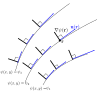
\includegraphics[width=0.75\textwidth]{./psi_streamlines}
 \caption{Relazione tra il campo e la funzione di corrente per un campo di velocità piano che soddisfa il vincolo di incomprimibilità. Il gradiente della funzione di corrente è perpendicolare in ogni punto al vettore velocità e, di conseguenza, le isolinee della funzione di corrente coincidono con le linee di corrente del campo di velocità.}\label{fig:streaml}
\end{figure}

\clearpage \newpage

\section{Tensore degli sforzi}


Il tensore degli sforzi $\mathbb{T}$ è un tensore del secondo ordine che descrive lo stato di sforzo all'interno del mezzo continuo e permette di legare il vettore sforzo $\bm{t_n}$ agente su una superficie elementare e il versore normale $\bh{n}$ alla superficie.
Si considera in un mezzo continuo non polare\footnote{
 All'interno del mezzo continuo, le particelle adiacenti si scambiano unicamente forze elementari, non momenti.
}, e si ricava il legame tra i vettori $\bm{t_n}$, $\bh{n}$ dalle condizioni di equilibrio del tetraedro di Cauchy. Siano $\bh{x}$, $\bh{y}$ e $\bh{z}$ i versori di un sistema di riferimento cartesiano centrato nel punto del continuo considerato e $\bm{t_x}$, $\bm{t_y}$ e $\bm{t_z}$ i vettori sforzo agenti sulle facce del tetraedro di area $dS_x$, $dS_y$ e $dS_z$ con le normali orientate come i rispettivi versori della base, come rappresentato in figura \ref{fig:tetraedroCauchy}. Sia $\bm{t_n}$ il vettore sforzo agente sulla faccia ``inclinata'' di area $dS$ del tetraedro di Cauchy, con normale $\bh{n}$.

\begin{figure}[h!]
\centering
 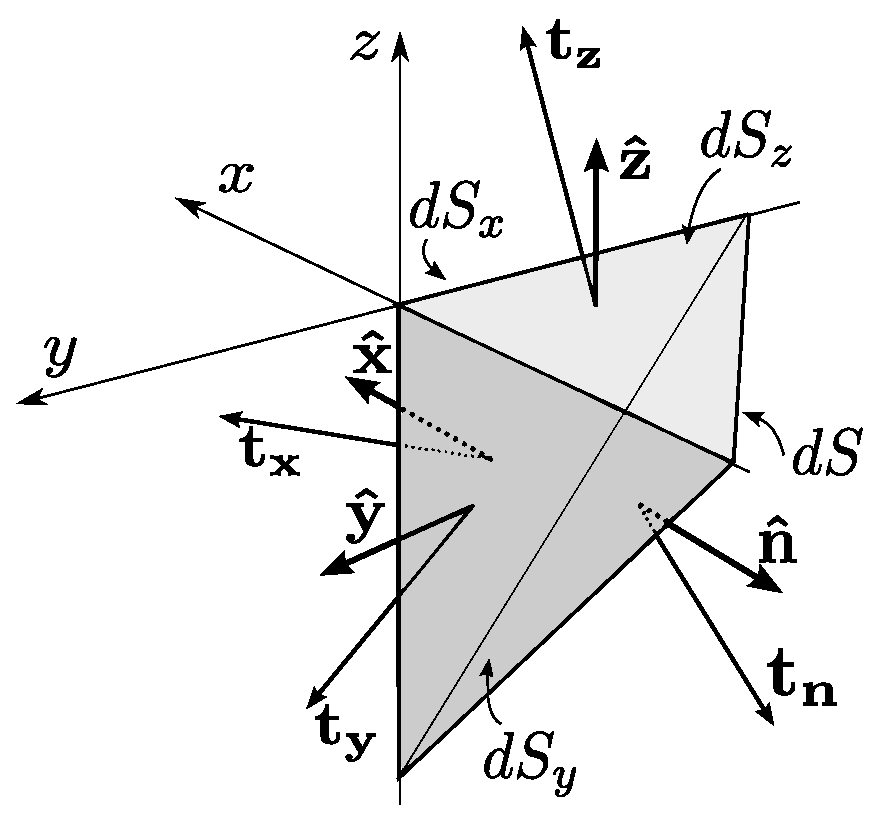
\includegraphics[width=0.60\textwidth]{./fig/cauchy}
\caption{tetraedro di Cauchy}\label{fig:tetraedroCauchy}
\end{figure}

Il legame tra le aree delle facce del tetraedro è
\begin{equation}\label{eqn:surfaces}
 dS = - \dfrac{dS_x}{n_x} = - \dfrac{dS_y}{n_y} = - \dfrac{dS_z}{n_z} ,
\end{equation}
avendo indicato con $n_i$ le componenti cartesiane del versore normale $\bh{n}$, tutte negative per come è stato definito il tetraedro.
Scriviamo il bilancio di massa e di quantità di moto del volume di controllo elementare $dV$ contenuto all'interno del tetraedro di Cauchy. Il bilancio di massa
\begin{equation}
 \f{d}{dt} \int_{dV} \rho + \oint_{\partial dV} \rho \bm{u} \cdot \bh{n} = 0 \ ,
\end{equation}
diventa
\begin{equation}\label{eqn:dV:mass}
\begin{aligned}
 0 = & \p{}{t}\big( \rho + O(d\ell) \big) dV
     + \big( \rho \bm{u} \cdot \bh{x} + O(d\ell) \big) dS_x
     + \big( \rho \bm{u} \cdot \bh{y} + O(d\ell) \big) dS_y \\
   & + \big( \rho \bm{u} \cdot \bh{z} + O(d\ell) \big) dS_z
     + \big( \rho \bm{u} \cdot \bh{n} + O(d\ell) \big) dS \ ,
\end{aligned}
\end{equation}
avendo scritto esplicitamente la dipendenza delle grandezze nel volume e sulle superfici da infinitesimi di ordine $O(d\ell)$, essendo $O(d\ell)$ l'ordine di grandezza delle dimensioni lineari del tetraedro di Cauchy, come ad esempio la lunghezza degli spigoli. Le superfici hanno ordine $O(dS) = O(d\ell^2)$, mentre il volume ha ordine $O(dV) = O(d\ell^3)$. Utilizzando le relazioni (\ref{eqn:surfaces}), facendo tendere $d\ell$ a zero, trascurando gli ifninitesimi di ordine superiore, i termini di ordine $O(d\ell^2)$ si riducono all'identità
\begin{equation}
 \bm{u} \cdot \bh{n} = u_x n_x + u_y n_y + u_z \ .
\end{equation}
Il bliancio di quantità di moto per il tetraedro di Cauchy
\begin{equation}
 \f{d}{dt} \int_V \rho \bm{u} + \oint_{\partial dV} \rho \bm{u} \bm{u} \cdot \bh{n} = \int_{dV} \rho \bm{g} + \oint_{\partial dV} \bm{t_n} \ ,
\end{equation}
diventa
\begin{equation}
\begin{aligned}
 & \p{}{t} \big( \rho \bm{u} + O(d\ell) \big)dV +
 \sum_{i \in \{x,y,z\}} \big( \rho \bm{u} \bm{u} \cdot \bh{x}_i + O(d\ell) \big)dS_i +
                \big( \rho \bm{u} \bm{u} \cdot \bh{n}   + O(d\ell) \big)dS   = \\
 & = \big( \rho \bm{g} + o(d\ell) \big) dV +
     \big( \bm{t_x} + O(d\ell) \big) dS_x +
     \big( \bm{t_y} + O(d\ell) \big) dS_y + \\
 & \hspace{4.5cm} + \big( \bm{t_z} + O(d\ell) \big) dS_z +
     \big( \bm{t_n} + O(d\ell) \big) dS \ .
\end{aligned}
\end{equation}
I termini ``più grandi'' sono infinitesimi di ordine $O(d\ell^2)$.
Utilizzando il bilancio di massa, non è difficile verificare che i termini di flusso di quantità di moto danno un contributo nullo di ordine $O(d\ell^2)$. I termini di volume sono infinitesimi di ordine $O(d\ell^3)$.
Facendo tendere $d\ell$ a zero e trascurando tutti gli infinitesimi di ordine superiore a $O(d\ell)$ si ottiene
\begin{equation}\label{eqn:dV:equil}
\begin{aligned}
 \bm{0} & = \bm{t_n} dS + \bm{t_x} dS_x + \bm{t_y} dS_y + \bm{t_z} dS_z = \\
  & = ( \bm{t_n} - \bm{t_x} n_x - \bm{t_y} n_y - \bm{t_z} n_z ) dS  \qquad \rightarrow \qquad \bm{t_n} = \bm{t_x} n_x + \bm{t_y} n_y + \bm{t_z} n_z \ .
\end{aligned}
\end{equation}
Se si esprimono i vettori utilizzando la base $\{\bh{x}, \, \bh{y}, \, \bh{z} \}$,
\begin{equation}\label{eqn:t:comp}
  \bm{t_i} = t_{ix} \bh{x} + t_{iy} \bh{y} + t_{iz} \bh{z} \ ,
\end{equation}
si può scrivere la relazione (\ref{eqn:dV:equil}) per trovare la relazione tra il versore $\bh{n}$ e il vettore sforzo $\bm{t_n}$
\begin{equation}
\begin{aligned}
  \bm{t_n} & = \bm{t_x} n_x + \bm{t_y} n_y + \bm{t_z} n_z \\ 
 & = n_x ( t_{xx} \bm{\hat{x}} + t_{xy} \bm{\hat{y}} +  t_{xz} \bm{\hat{z}} ) % + \\
   + n_y ( t_{yx} \bm{\hat{x}} + t_{yy} \bm{\hat{y}} +  t_{yz} \bm{\hat{z}} ) % + \\
   + n_z ( t_{zx} \bm{\hat{x}} + t_{zy} \bm{\hat{y}} +  t_{zz} \bm{\hat{z}} ) = \\
 & = ( \bh{n} \cdot \bh{x} ) ( t_{xx} \bm{\hat{x}} + t_{xy} \bm{\hat{y}} +  t_{xz} \bm{\hat{z}} )% + \\
   + ( \bh{n} \cdot \bh{y} ) ( t_{yx} \bm{\hat{x}} + t_{yy} \bm{\hat{y}} +  t_{yz} \bm{\hat{z}} )% + \\
   + ( \bh{n} \cdot \bh{z} ) ( t_{zx} \bm{\hat{x}} + t_{zy} \bm{\hat{y}} +  t_{zz} \bm{\hat{z}} ) = \\
%   & = ( \bm{n} \cdot \bm{\hat{x}} ) \bm{t_x} + 
%       ( \bm{n} \cdot \bm{\hat{y}} ) \bm{t_y} + 
%       ( \bm{n} \cdot \bm{\hat{z}} ) \bm{t_z} = \\
    & = \bh{n} \cdot ( t_{xx} \bm{\hat{x}} \otimes \bm{\hat{x}} + 
                       t_{xy} \bm{\hat{x}} \otimes \bm{\hat{y}} +
                       t_{xz} \bm{\hat{x}} \otimes \bm{\hat{z}} + \\
            & \qquad + t_{yx} \bm{\hat{y}} \otimes \bm{\hat{x}} + 
                       t_{yy} \bm{\hat{y}} \otimes \bm{\hat{y}} +
                       t_{yz} \bm{\hat{y}} \otimes \bm{\hat{z}} + \\
            & \qquad + t_{zx} \bm{\hat{z}} \otimes \bm{\hat{x}} + 
                       t_{zy} \bm{\hat{z}} \otimes \bm{\hat{y}} +
                       t_{zz} \bm{\hat{z}} \otimes \bm{\hat{z}} ) =
     \bm{\hat{n}} \cdot \mathbb{T}  \ ,
\end{aligned}  
\end{equation}
avendo utilizzato l'identità $(\bm{a} \cdot \bm{b})\bm{c} = \bm{a} \cdot (\bm{b}\otimes\bm{c})$, per isolare il versore $\bh{n}$ dal tensore degli sforzi $\mathbb{T}$. Avendo utilizzato la definizione (\ref{eqn:t:comp}) delle componenti cartesiane dei vettori dello sforzo agente sulle facce del tetraedro di Cauchy, il primo indice delle componenti del tensore degli sforzi indica la faccia sulla quale agisce lo sforzo, il secondo indice la sua componente cartesiana, cosicché la componente $t_{ij}$ indica la componente cartesiana $j$-esima agente sulla $i$-esima faccia del tetraedro di Cauchy.
%
\newline \noindent
\textbf{Osservazione 1.} Utilizzando le convenzioni scelte in precedenza, il vettore sforzo si ottiene con la relazione
\begin{equation}
 \bm{t_n} = \bh{n} \cdot \mathbb{T} \qquad , \qquad t_{n,i} = n_j t_{ji} \ ,
\end{equation}
che in generale differisce dall'operazione $\mathbb{T} \cdot \bh{n}$, la cui $i$-esima componente cartesiana è $n_j t_{ij}$.
%
\newline \noindent
\textbf{Osservazione 2.} Se il tensore $\mathbb{S}$ è simmetrico (e quindi le sue componenti con indici misti sono uguali, $S_{ij} = S_{ji}$), la moltiplicazione a sinista o a destra di un vettore tramite il prodotto ``punto'' dà lo stesso risultato,
\begin{equation}
 \bm{a} \cdot \mathbb{S} = \mathbb{S} \cdot \bm{a} \qquad , \qquad 
 a_j S_{ji} = S_{ij} a_j \ .
\end{equation}
%
\newline \noindent
\textbf{Osservazione 3.} Il tensore degli sforzi per mezzi continui non polari è simmetrico. Questo permette di ottenere la corretta relazione tra versore normale alla superficie e vettore sforzo, anche in seguito ad alcune imprecisioni nell'utilizzo delle operazioni tensoriali, come uno scambio di indici nel tensore degli sforzi.
%
\newline \noindent
\textbf{Osservazione 4.} Non è stata prestata mai attenzione alla posizione degli indici poiché si è lavorato sempre con basi ortonormali, come la base cartesiana.
%
\newline \noindent
\textbf{Osservazione 5.} \'E possibile utilizzare altre convenzioni nella definizione delle componenti dei vettori sforzo agenti sulle facce del tetraedro di Cauchy, che portano a una diversa interpretazione degli indici e alla rappresentazione della relazione di Cauchy.





\clearpage \newpage

\section{Equazione della quantità di moto e curvatura delle linee di corrente}

L'equazione della quantità di moto è
\begin{equation}
 \rho \left\{ \frac{\partial \bm{u}}{\partial t} +
   \left( \bm{u} \cdot \bm{\nabla} \right) \bm{u} \right\} = 
   \bm{\nabla} \cdot \mathbb{T} + \bm{f}
\end{equation}
dove con $\mathbb{T}$ è stato indicato il tensore degli sforzi,
 che per un fluido newtoniano è $\mathbb{T} = -p \mathbb{I} + \mathbb{S}$
 con $\mathbb{S} = 2 \mu \mathbb{D} + \lambda \left( 
 \bm{\nabla} \cdot \bm{u} \right) \mathbb{I}$ e $\mathbb{D} = \frac{1}{2}
 \left[ \bm{\nabla}\bm{u} + \bm{\nabla}^T \bm{u} \right]$ il tensore
 velocità di deformazione, parte simmetrica del gradiente della velocità.
%
Introducendo la derivata materiale, si ritrova una forma ``familiare''
 del secondo principio della dinamica
\begin{equation}
 \rho\frac{D\bm{u}}{D t} = \bm{\nabla} \cdot \mathbb{T} + \bm{f}
  \qquad \Rightarrow \qquad
 \rho\bm{a} = \bm{\nabla} \cdot \mathbb{T} + \bm{f}
\end{equation}
%
\paragraph{Richiami di geometria delle curve nello spazio.}
Una curva è un luogo di punti che può essere parametrizzato tramite un
 parametro solo.
La parametrizzazione $\bm{r}(t)$ della curva $\bm{r}$ è definita regolare 
 se $d\bm{r}/dt \ne 0$. Si definisce poi una parametrizzazione regolare
 particolare, l'ascissa curvilinea $s$ tale per cui $\left| d\bm{r}(s)/ds
 \right| = 1, \forall s \in (a,b)$.

\noindent 
Nel seguito si introduce brevemente la \textbf{terna di Frenet} 
 $\left\{\bm{\hat{t}}, \bm{\hat{n}}, \bm{\hat{b}} \right\}$, formata
 dai versori tangente, normale e binormale, in funzione dell'ascissa
 curvilinea.
%
Si dimostra che
\begin{equation}
 \bm{\hat{t}}(s) = \dfrac{d\bm{r}}{ds}
\end{equation}
%
La derivata seconda della posizione $\bm{r}$, cioè la derivata prima del
 versore tangente $\bm{\hat{t}}$ è legata al versore normale
 $\bm{\hat{t}}$, tramite la curvatura $k = \left| \frac{d\bm{\hat{t}}}{
 ds} \right|$.
\begin{equation}
 \bm{\hat{n}} = \dfrac{\frac{d\bm{\hat{t}}}{ds}}
    {\left|\frac{d\bm{\hat{t}}}{ds} \right|} 
  \qquad \Rightarrow \qquad
 \dfrac{d\bm{\hat{t}}}{ds} = k \bm{\hat{n}}
\end{equation}
%
Il versore binormale è definito a completare la terna ortonormale 
 destrorsa
\begin{equation}
 \bm{\hat{b}} = \bm{\hat{t}} \times \bm{\hat{n}} 
\end{equation}
%
Per completezza e senza troppo sforzo si calcolano anche le derivate 
 di tali versori, ricordando che hanno modulo unitario e costante,
 e formano una terna ortogonale in ogni punto, introducendo la definizione
 della torsione $\tau = \frac{d \bm{\hat{n}}}{ds}\cdot \bm{b}$.
\begin{equation}
\begin{aligned}
& \qquad \qquad \qquad \qquad \qquad \qquad \qquad \qquad 
  \qquad \qquad \qquad \qquad \quad
 \frac{d \bm{\hat{t}}}{ds} = k \bm{\hat{n}} \\
& \begin{cases}
 \bm{\hat{n}}'\cdot \bm{\hat{n}} = 0 \\
 \bm{\hat{n}}'\cdot \bm{\hat{t}}+\bm{\hat{t}}'\cdot \bm{\hat{n}} = 0 \\
 \bm{\hat{n}}'\cdot \bm{\hat{b}} = \tau \\
 \end{cases} \Rightarrow \quad
 \begin{cases}
 \bm{\hat{n}}'\cdot \bm{\hat{n}} = 0   \\
 \bm{\hat{n}}'\cdot \bm{\hat{t}} = -k  \\
 \bm{\hat{n}}'\cdot \bm{\hat{b}} = \tau \\
 \end{cases} \qquad \quad \quad \Rightarrow \quad 
  \frac{d \bm{\hat{n}}}{ds} = - k \bm{\hat{t}} + \tau \bm{\hat{b}} \\
& \begin{cases}
 \bm{\hat{b}}'\cdot \bm{\hat{b}} = 0 \\
 \bm{\hat{b}}'\cdot \bm{\hat{t}} + \bm{\hat{t}}'\cdot \bm{\hat{b}} = 0 \\
 \bm{\hat{b}}'\cdot \bm{\hat{n}} + \bm{\hat{n}}'\cdot \bm{\hat{b}} = 0 \\
 \end{cases} \Rightarrow \quad
 \begin{cases}
 \bm{\hat{b}}'\cdot \bm{\hat{b}} = 0 \\
 \bm{\hat{b}}'\cdot \bm{\hat{t}} = -\bm{\hat{t}}'\cdot \bm{\hat{b}} = 0 \\
 \bm{\hat{b}}'\cdot \bm{\hat{n}} = -\bm{\hat{n}}'\cdot \bm{\hat{b}} = -k\\
 \end{cases} \Rightarrow \quad
  \frac{d \bm{\hat{b}}}{ds} = - \tau \bm{\hat{n}} \\
\end{aligned}
\end{equation}
%
Se la parametrizzazione regolare della curva non è l'ascissa curvilinea,
 si può ricavare
\begin{equation}
 \frac{d\bm{r}}{dt} = \frac{ds}{dt}\frac{d\bm{r}}{ds} = 
  v \bm{\hat{t}}
\end{equation}
dove si è introdotto il modulo $v$ di quella che sarà la velocità $\bm{v}$
 quando $\bm{r}$ e $t$ saranno spazio e tempo.
In maniera analoga
\begin{equation}
 \frac{d\bm{\hat{t}}}{dt} = \frac{ds}{dt}\frac{d\bm{\hat{t}}}{ds} = 
  v k \bm{\hat{n}}
\end{equation}
 %
Se $\bm{r}$ e $t$ sono spazio e tempo, la velocità e l'accelerazione di un
 punto che ha come legge oraria $\bm{r}(t)$ sono
\begin{equation}
 \begin{aligned}
  \bm{v} & = \frac{d\bm{r}}{dt} = \frac{ds}{dt}\frac{d\bm{r}}{ds} = 
    v \bm{\hat{t}} \\
  \bm{a} & = \frac{d\bm{v}}{dt} =
   \frac{dv}{dt} \bm{\hat{t}} + v \frac{d\bm{\hat{t}}}{dt} =
   \frac{dv}{dt} \bm{\hat{t}} + v^2 k \bm{\hat{n}}
 \end{aligned}
\end{equation}
%
\begin{minipage}{0.60\textwidth}
\paragraph{Ritorno al bilancio della quantità di moto.} Inserendo la
 forma dell'accelerazione nell'equazione della quantità di moto e 
 proiettando lungo i versori della terna di Frenet
\begin{equation}
 \begin{cases}
  \rho \frac{dv}{dt} =  \bm{\hat{t}} \cdot \left(
     \bm{\nabla} \cdot \mathbb{T} + \bm{f} \right) \\
  \rho v^2 k = \bm{\hat{n}} \cdot \left(
     \bm{\nabla} \cdot \mathbb{T} + \bm{f} \right) \\
  0 = \bm{\hat{b}} \cdot \left(
     \bm{\nabla} \cdot \mathbb{T} + \bm{f} \right) \\
 \end{cases}
\end{equation}
L'analisi per componenti locali dell'equazione della quantità di moto permette di riconoscere che:
\end{minipage}
\hfill
\begin{minipage}{0.40\textwidth}
\begin{center}
   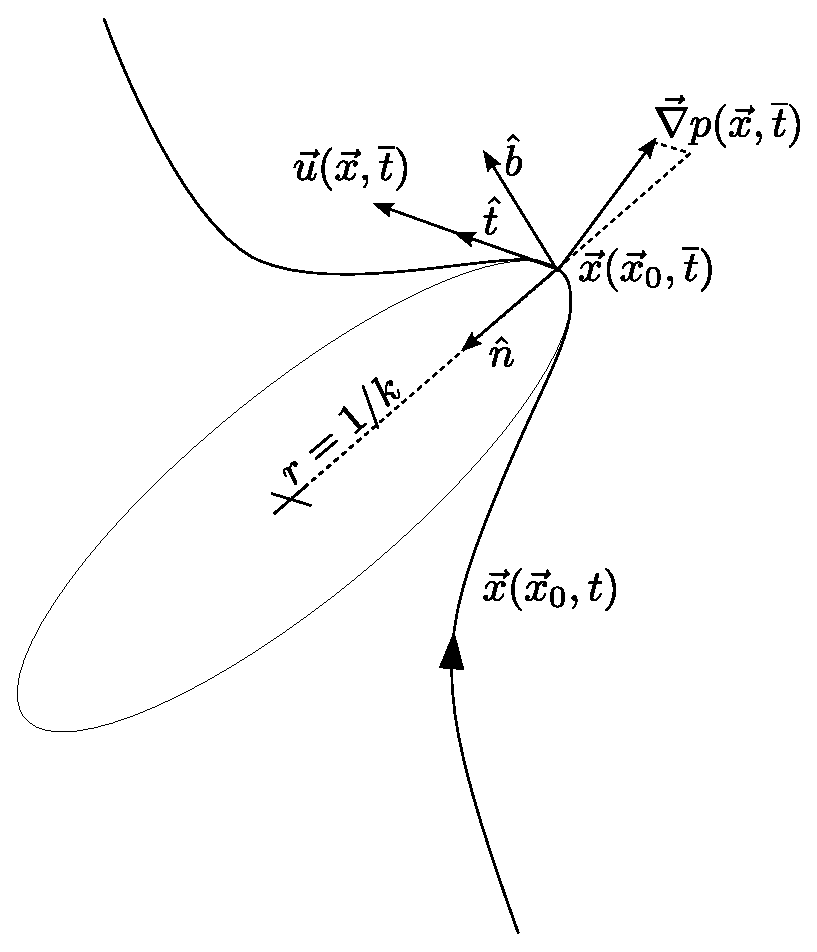
\includegraphics[width=1.0\textwidth]{./fig/frenet.eps}
\end{center}
\end{minipage}
\begin{itemize}
 \item la proiezione del termine forzante lungo la tangente alla traiettoria è la responsabile dell'accelerazione tangenziale della particella materiale;
 \item la proiezione del termine forzante lungo la normale alla traiettoria è la responsabile dell'accelerazione centripeta della particella maetriale e, di conseguenza, della curvatura della traiettoria;
 \item la proiezione della forzante lungo la direzione binormale è nulla.
\end{itemize}

\noindent
In assenza di forze di volume ($\bm{f}=0$) e sforzi viscosi
($\mathbb{T}=\mathbb{S}-p\mathbb{I}=-p\mathbb{I}$):
\begin{equation}
 \begin{cases}
  \rho \frac{dv}{dt} = - \bm{\hat{t}} \cdot \bm{\nabla} p \\
  \rho v^2 k         = - \bm{\hat{n}} \cdot \bm{\nabla} p \\
  0                  = - \bm{\hat{b}} \cdot \bm{\nabla} p \\
 \end{cases}
\end{equation}
%
e quindi:
\begin{itemize}
 \item l'accelerazione tangenziale è proporzionale alla proiezione del gradiente di pressione in direzione tangente alla tratiettoria;
 \item l'accelerazione centripeta, $v^2/r = v^2 k$, è proporzionale alla proiezione del gradiente di pressione in direzione normale alla tratiettoria. Il termine $\rho v^2 k$ è sempre positivo poichè prodotto di quantità positive: la curvatura di una linea è non negativa per come è definita, la densità è positiva, il modulo di un vettore è anch'esso non negativo. Il prodotto scalare tra la normale e il gradiente della pressione (derivata direzionale della pressione in direzione $\bm{\hat{n}}$) deve quindi essere negativo. La pressione quindi diminuisce, andando verso il centro del cerchio osculatore. Sempre dalla seconda equazione è immediato notare che la curvatura della traiettoria è proporzionale alla componente del gradiente di pressione lungo il versore normale;
 \item la proiezione del gradiente di pressione in direzione binormale a una traiettoria è nullo.
\end{itemize}
% Un'analisi della componente normale permette di ricavare, \textbf{sotto le
%  ipotesi fatte}, il legame tra la curvatura delle traiettorie delle
%  particelle fluide e il gradiente del campo di pressione.
% Il termine a sinistra dell'uguale è positivo
% La componente tangente fa aumentare 
%  il modulo della velocità, mentre la componente binormale deve essere nulla.
%Essendo il versore $\bm{\hat{n}}$ diretto verso il centro del cerchio
% osculatore (in parole povere è diretta verso l'interno della curva),
% la curvatura $k$ positiva, segue che la pressione deve diminuire lungo 
% $\bm{\hat{n}}$, cioè aumenta all'allontanarsi dal cerchio del centro
% osculatore (in parole altrettanto povere, ``verso l'esterno'').
%\textit{(Nemmeno a dirlo, la densità $\rho$ è positiva e il quadrato
%  del modulo della velocità $v^2$ è positivo.)}
%\noindent
%Dalla componente lungo $\bm{\hat{n}}$ si nota che il legame tra 
% la componente del gradiente della pressione in quella direzione è
% \textbf{proporzionale} alla curvatura della traiettoria della particella
% fluida.


\clearpage \newpage

\section{Teoremi di Bernoulli ed equazione della vorticità}
Per fluidi incomprimibili o barotropici (per i quali la pressione è funzione solo della densità), il teorema di Bernoulli si ottiene dal bilancio della quantità di moto. Si elencano qui tre forme del teorema di Bernoulli, ognuna caratterizzata da diverse ipotesi.
%
Tramite l'identità vettoriale
\begin{equation}
  \bm{\nabla} (\bm{a} \cdot \bm{b}) = (\bm{a} \cdot \bm{\nabla}) \bm{b} +  (\bm{b} \cdot \bm{\nabla}) \bm{a} + \bm{a} \times (\bm{\nabla} \times \bm{b}) + \bm{b} \times (\bm{\nabla} \times \bm{a}),
\end{equation}
applicata al termine convettivo $(\bm{u} \cdot \bm{\nabla}) \bm{u}$, è possible ottenere la forma del Crocco dell'equazione della quantità di moto
\begin{equation}\label{eqn:bilanci:crocco}
\begin{aligned}
 & \p{\bm{u}}{t} + (\bm{u} \cdot \bm{\nabla}) \bm{u} - \nu \Delta \bm{u} + \bm{\nabla} P = \bm{g}  & \\ &  &  \bigg( (\bm{u} \cdot \bm{\nabla})\bm{u} = \bm{\nabla} \f{\bm{u} \cdot \bm{u}}{2} + (\bm{\nabla} \times \bm{u}) \times \bm{u} \bigg) \\
 & \rightarrow \p{\bm{u}}{t} + \bm{\nabla} \frac{|\bm{u}|^2}{2} + \bm{\omega} \times \bm{u} - \nu \Delta \bm{u} + \bm{\nabla} P = \bm{g} , & \\
\end{aligned}
\end{equation}
avendo indicato con $P$ il potenziale termodinamico, $P = $ che si riduce al rapporto $p/\rho$ nel caso di densità costante e con $\bm{g}$ le forze per unità di massa.
\paragraph{Prima forma del teorema di Bernoulli}
Nel caso di fluido non viscoso, incomprimibile o barotropico, in regime stazionario ($\partial / \partial t \equiv 0$), con forze di massa conservative $\bm{g} = -\bm{\nabla} \chi$, il trinomio di Bernoulli $|\bm{u}|^2/2 + P + \chi$ è costante lungo le linee di corrente e le linee vorticose, cioè
\begin{equation}
 \bm{\hat{t}} \cdot \bm{\nabla} \left( \frac{|\bm{u}|^2}{2} + P + \chi \right) = 0 ,
\end{equation}
con $\bm{\hat{t}}$ versore tangente alle linee di corrente o alle linee vorticose. Infatti, il termine $\bm{\omega} \times \bm{u}$ nell'equazione della quantità di moto nella forma di Crocco (\ref{eqn:bilanci:crocco}) è perpendicolare in ogni punto del dominio alle linee di corrente ($\bm{\hat{t}}$ parallelo al campo di velocità $\bm{u}$) e alle linee vorticose ($\bm{\hat{t}}$ parallelo al campo di vorticità $\bm{\omega}$): moltiplicando scalarmente l'equazione (\ref{eqn:bilanci:crocco}) scritta per un fluido non viscoso ($\nu = 0$) per il versore $\bm{\hat{t}}$ , il prodotto scalare $\bm{\hat{t}} \cdot (\bm{\omega} \times \bm{u})$ è identicamente nullo.
\paragraph{Seconda forma del teorema di Bernoulli}
Nella corrente irrotazionale ($\bm{\omega} = \bm{0}$) di un fluido non viscoso, incomprimibile o barotropico, in regime stazionario, con forze di massa conservative $\bm{g} = -\bm{\nabla} \chi$, il trinomio di Bernoulli $|\bm{u}|^2/2 + P + \chi$ è costante in tutto il dominio, cioè
\begin{equation}
 \bm{\nabla} \left( \frac{|\bm{u}|^2}{2} + P + \chi \right) = 0  \quad \rightarrow \quad 
  \frac{|\bm{\nabla} \phi|^2}{2} + P + \chi = C.
\end{equation}
\paragraph{Terza forma del teorema di Bernoulli}
Nella corrente irrotazionale ($\bm{\omega} = \bm{0}$) di un fluido non viscoso, incomprimibile o barotropico, in un dominio semplicemente connesso (nel quale è quindi possibile definire il potenziale cinetico $\phi$, t.c. $\bm{u} = \nabla \phi$, con forze di massa conservative $\bm{g} = -\bm{\nabla} \chi$, il quadrinomio di Bernoulli $\partial \phi / \partial t + |\bm{u}|^2/2 + P + \chi$ è uniforme (costante in spazio, in generale \textbf{non} in tempo) in tutto il dominio, cioè
\begin{equation}
 \bm{\nabla} \left(\p{\phi}{t} + \frac{|\bm{\nabla} \phi|^2}{2} + P + \chi \right) = 0  \quad \rightarrow \quad 
 \p{\phi}{t} + \frac{|\bm{\nabla} \phi|^2}{2} + P + \chi = C(t).
\end{equation}

\paragraph{Teoremi di Bernoulli per fluidi viscosi incomprimibili}
Mentre la prima forma del teorema di Bernoulli non è valida se non viene fatta l'ipotesi di fluido non viscoso\footnote{Moltiplicando scalarmente l'equazione (\ref{eqn:bilanci:crocco}) per il versore $\bm{\hat{t}}$, il termine $\bm{\hat{t}}\cdot \nu \Delta \bm{u}$ non si annulla. Rimane quindi
\begin{equation}
 \bm{\hat{t}} \cdot \bm{\nabla} \left( \frac{|\bm{u}|^2}{2} + P + \chi \right) - \nu \bm{\hat{t}} \cdot \Delta \bm{u} = 0 
\end{equation}
}, la seconda e la terza forma sono ancora valide per fluidi viscosi incomprimibili. Infatti, usando l'identità vettoriale
\begin{equation}
 \Delta \bm{u} = \bm{\nabla} (\bm{\nabla}\cdot \bm{u})
  - \bm{\nabla} \times (\bm{\nabla} \times \bm{u}) ,
\end{equation}
si scopre che il laplaciano del campo di velocità per correnti irrotazionali ($\bm{\nabla} \times \bm{u} = \bm{0}$) di fluidi incomprimibili ($\bm{\nabla} \cdot \bm{u} = 0$) è nullo.
%
\begin{remark}
L'ipotesi di fluido non viscoso non è direttamente necessaria per la seconda e la terza forma del teorema di Bernoulli, ma lo diventa tramite l'ipotesi di corrente irrotazionale. Sotto opportune ipotesi sulla corrente asintotica, verificate in molti casi di interesse aeronautico, si dimostra che (quasi) tutto il campo di moto è  irrotazionale solo se viene fatta l'ipotesi di fluido non viscoso. Questo modello viene utilizzato per studiare correnti di interesse aeronautico, nelle quali gli effetti della viscosità sono (quasi ovunque) trascurabili: un esempio è la corrente, uniforme a monte, che investe un corpo aerodinamico a bassi angoli di incidenza (corpo affusolato, attorno al quale non si verifichino separazioni) per alti numeri di Reynolds: in queste correnti, le zone vorticose sono confinate in regioni di spessore sottile (strato limite sulla superficie dei corpi solidi e scie libere).
\end{remark}





\clearpage \newpage

\section{Teorema di Kutta--Jukowski}

Il teorema di Kutta--Jukowski lega la circolazione attorno a un corpo alla portanza generata, nelle ipotesi di correnti incomprimibili, non viscose, irrotazionali.
Utilizzando i bilanci integrali di massa e di quantità di moto, ricaveremo il teorema di Kutta--Jukowski per un problema bidimensionale stazionario.
Utilizziamo un sistema di coordinate cartesiano, con l'asse $x$ orientato come la velocità asintotica $\bm{U}_{\infty} = U_{\infty} \bm{\hat{x}}$ che investe il corpo. Scriviamo poi il campo di velocità come la somma della velocità asintotica e una velocità \textit{di preturbazione} $\bm{u}'(\bm{r})$,
\begin{equation}\label{eqn:vel:dec}
 \bm{u}(\bm{r}) = \bm{U}_{\infty} + \bm{u}'(\bm{r}) \ .
\end{equation}
L'unico ``atto di fede'' che vi viene richiesto riguarda l'andamento asintotico della velocità di perturbazione all'infinito. Si può dimostrare che la velocità di perturbazione è proporzionale all'inverso della distanza dal corpo,
\begin{equation}
 |\bm{u}'(\bm{r})| \sim \dfrac{1}{|\bm{r}|} \quad, \qquad |\bm{r}| \rightarrow \infty \ .
\end{equation}
Utilizzando il bilancio integrale di quantità di moto per il volume di controllo euleriano $V$ rappresentato in figura {\color{red} \dots}, si può valurare la forza esercitata dal fluido sul corpo,
\begin{equation}
 \bm{R} = - \oint_S \rho \bm{u} \bm{u} \cdot \bm{\hat{n}} - \oint_S P \bm{\hat{n}} \ ,
\end{equation}
Nell'ipotesi che la corrente sia irrotazionale, si può utilizzare il teorema di Bernoulli per valutare il campo di pressione in funzione della velocità e delle condizioni asintotiche,
\begin{equation}
 P = P_{\infty} + \dfrac{1}{2} \rho U_{\infty}^2 - \dfrac{1}{2} \rho |\bm{u}|^2 \ ,
\end{equation}
e riscrivere l'espressione della forza agente sul corpo come,
\begin{equation}
 \bm{R} = - \oint_S \rho \bm{u} \bm{u} \cdot \bm{\hat{n}} + \oint_S \dfrac{1}{2} \rho |\bm{u}|^2 \bm{\hat{n}} \ ,
\end{equation}
avendo semplificato gli integrali nulli su una superficie chiusa di una quantità costante moltiplicata per il versore normale.

\begin{figure}[h!]
\centering
 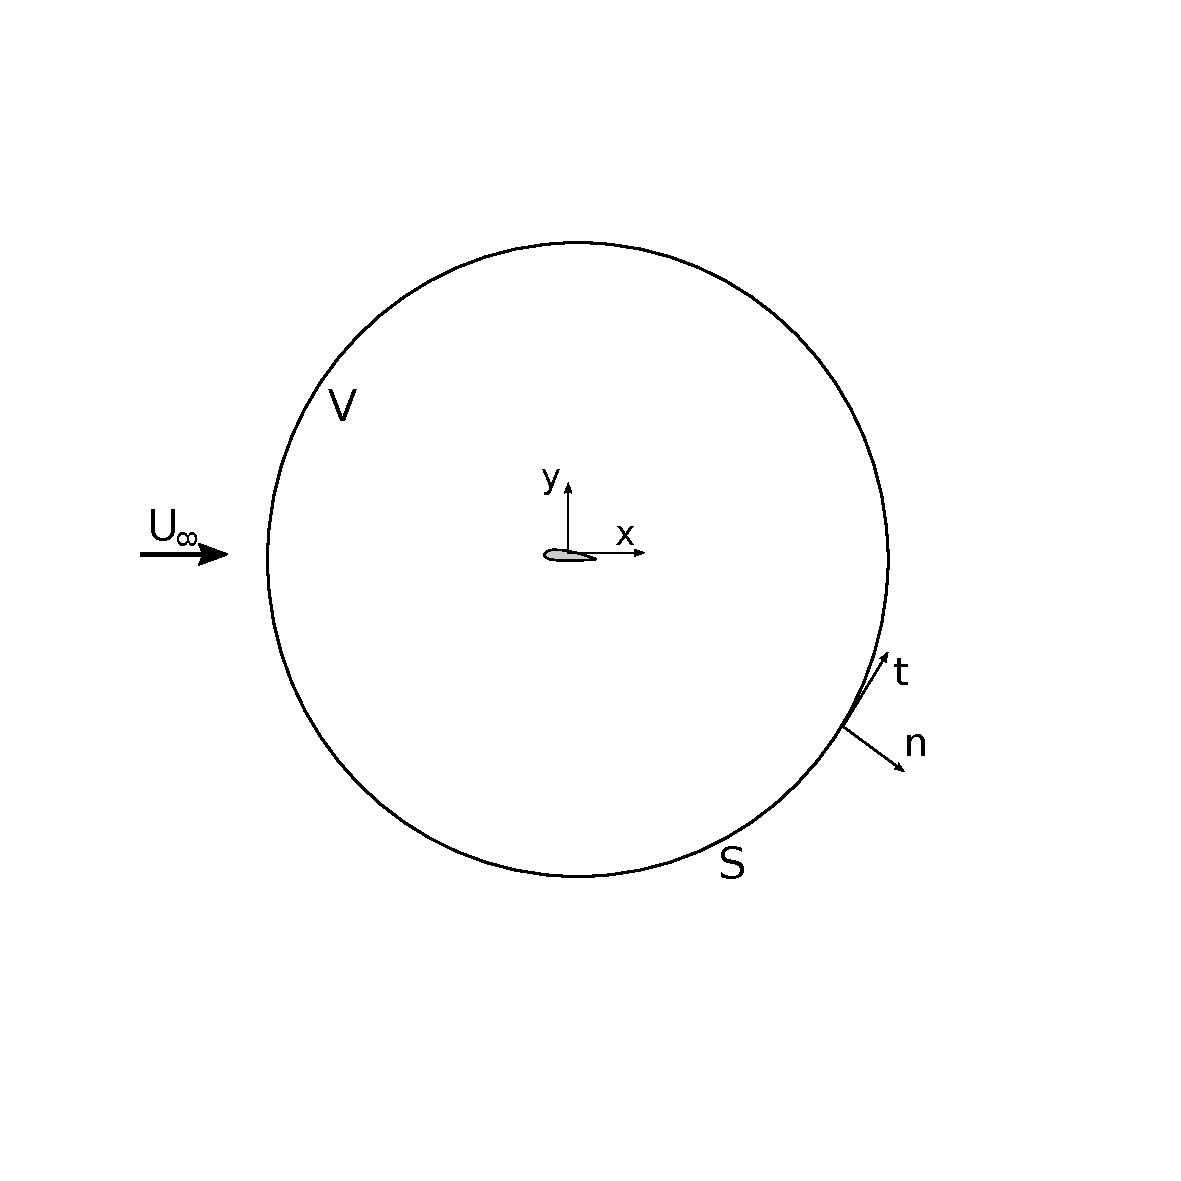
\includegraphics[width=0.75\textwidth, trim= 40 100 100 100, clip]{./fig/kj}
\caption{volume di controllo per la dimostrazione del teorema di Kutta--Jukowski.}\label{fig:kj}
\end{figure}

A questo punto, si può utilizzare l'espressione della velocità (\ref{eqn:vel:dec}), per manipolare gli integrali,
\begin{equation}\label{eqn:kj:1}
\begin{aligned}
 \bm{R} & = - \oint_S \rho \bm{U}_{\infty} \bm{u} \cdot \bm{\hat{n}}
            - \oint_S \rho \bm{u}'         \bm{u} \cdot \bm{\hat{n}} \\
   & \qquad + \oint_S \dfrac{1}{2} \rho U^2_{\infty}  \bm{\hat{n}}
            + \oint_S \rho \bm{U}_{\infty} \cdot \bm{u}' \bm{\hat{n}}
            + \oint_S \rho |\bm{u}'|^2 \bm{\hat{n}} \ .
\end{aligned}
\end{equation}
Il primo integrale è nullo per il bilancio integrale della massa, poiché
\begin{equation}
  \oint_S \rho \bm{U}_{\infty} \bm{u} \cdot \bm{\hat{n}} = 
  \rho \bm{U}_{\infty} \oint_S \bm{u} \cdot \bm{\hat{n}} = 0 \ ,
\end{equation}
se il corpo non inietta fluido nel dominio. Il terzo integrale è nullo.
Il secondo integrale può essere riscritto come
\begin{equation}
- \oint_S \rho \bm{u}'         \bm{u} \cdot \bm{\hat{n}} = 
- \oint_S \rho \bm{u}' \bm{U}_{\infty}\cdot \bm{\hat{n}} 
- \oint_S \rho \bm{u}' \bm{u}'        \cdot \bm{\hat{n}} \ .
\end{equation}
Quando si fa tendere la superficie $S$ all'infinito, la dimensione del dominio di integrazione tende all'infinito come $r$. Poiché $|\bm{u}'| \sim 1/r$ quando $r \rightarrow \infty$, gli integrali quadratici in $\bm{u}'$ tendono a zero.

Rimettendo insieme tutti i pezzi dell'equazione (\ref{eqn:kj:1}), quando $r \rightarrow \infty$, si ottiene
\begin{equation}
 \bm{R} = - \oint_S \rho \bm{u}' \bm{U}_{\infty}\cdot \bm{\hat{n}} 
          + \oint_S \rho \bm{U}_{\infty} \cdot \bm{u}' \bm{\hat{n}} \ .
\end{equation}
Questa espressione può essere manipolata utilizzando l'identità vettoriale $\bm{a} \times (\bm{b} \times \bm{c} ) = (\bm{a} \cdot \bm{c}) \bm{b} - (\bm{a} \cdot \bm{b}) \bm{c}$, per scrivere
\begin{equation}
 \bm{R} = - \rho \bm{U}_\infty \times \oint_S \bm{u}' \times \bm{\hat{n}} \ .
\end{equation}
In due dimensioni, il versore normale alla superficie può essere espresso in funzione del versore tangente,
\begin{equation}
 n_x = t_y \quad , \quad n_y = - t_x \ ,
\end{equation}
e quindi è possibile riscrivere il prodotto vettore $\bm{u}' \times \bm{\hat{n}} = -\bm{\hat{z}} \,(\bm{u}' \cdot \bm{\hat{t}})$, e la risultante sul corpo
\begin{equation}
 \bm{R} = \rho \bm{U}_\infty \times \bm{\hat{z}} \, \oint_S \bm{u}' \cdot \bm{\hat{t}} \ .
\end{equation}
Si può sommare all'integrale il termine nullo $\oint_S \bm{U}_{\infty} \cdot \bm{\hat{t}}$ per ottenere\begin{equation}
 \bm{R} = \rho \bm{U}_\infty \times \bm{\hat{z}} \, \oint_S \bm{u} \cdot \bm{\hat{t}} \ ,
\end{equation}
svolgere il prodotto vettoriale $\bm{U}_{\infty} \times \bm{\hat{z}} = - U_{\infty} \bm{\hat{y}}$, e riconoscere la definizione della circolazione attorno al corpo,
\begin{equation}
 \Gamma = \oint_S \bm{u} \cdot \bm{\hat{t}} \ ,
\end{equation}
per ricavare l'espressione del teorema di Kutta--Jukowski,
\begin{equation}
 \bm{R} = -\rho U_{\infty} \Gamma \bm{\hat{y}} \ .
\end{equation}




\clearpage \newpage

\section{Cenni sulla similitudine}

In questo paragrafo viene ripreso il concetto di \textbf{scala caratteristica} (di lunghezza, di tempo, \dots) di un sistema nell'ambito della similitudine, per determinare il numero di parametri adimensionali caratteristici del problema, grazie al teorema di Buckingham.
Cerchiamo di raccordare il processo rigoroso di adimensionalizzazione delle equazioni con un approccio più euristico che valuta ``intuitivamente'' quali sono le grandezze significative indipendenti che influenzano il problema.

\subsection{Adimensionalizzazione delle equazioni di Navier--Stokes}
L'adimensionalizzazione delle equazioni di Navier--Stokes per una corrente incomprimibile, a densità e viscosità uniforme,
\begin{equation}
\begin{cases}
 \rho\p{\bm{u}}{t} + \rho ( \bm{u} \cdot \bm{\nabla} ) \bm{u} 
 - \mu\Delta \bm{u} - \bm{\nabla} p = 0 \ , \\
 \bm{\nabla} \cdot \bm{u} = 0 \ ,
\end{cases}
\end{equation}
viene svolta esprimendo ogni grandezza fisica che compare nelle equazioni come prodotto di una grandezza dimensionale di riferimento e la grandezza adimensionalizzata,
\begin{equation}
\begin{aligned}
 \bm{x} & = L \bm{x}^* \\  
     t  & = T    {t}^* \\
 \bm{u} & = U \bm{u}^* \\
     p  & = P    {p}^* \\
 \mu    & = \mu  \mu^* \ , \quad  \mu^* = 1 \\
 \rho   & = \rho\rho^* \ , \quad \rho^* = 1 \ ,
\end{aligned}
\end{equation}
avendo scelto come grandezza dimensionale di riferimento per i parametri uniformi (densità e viscosità dinamica) la grandezza stessa, poiché non ha senso (o almeno, io non ne vedo il motivo) scegliere un altro valore di riferimento. Con questa scelta, la densità e la viscosità dinamica adimensionali hanno valore unitario.
L'operatore nabla viene infine espresso come,
\begin{equation}
 \bm{\nabla} = \dfrac{1}{L} \bm{\nabla}^* \ ,
\end{equation}
ricordandosi che contiene le derivate spaziali. Le equazioni di Navier--Stokes contengono $A=6$ grandezze fisiche,
\begin{equation}
 \bm{u}, \ p, \ \bm{x}, \ t, \ \rho, \ \mu \ ,
\end{equation}
e $B=3$ dimensioni fisiche,
\begin{equation}
 \text{massa, lunghezza, tempo} \ ,
\end{equation}
quindi il problema è completamente caratterizzato da $C=A-B = 3$ numeri adimensionali per il teorema $\pi$ di Buckingham.

\vspace{0.2cm}
\noindent
Le equazioni di Navier--Stokes diventano
\begin{equation}
\begin{cases}
 \dfrac{U}{T} \p{\bm{u}^*}{t^*} + \dfrac{U^2}{L} ( \bm{u}^* \cdot \bm{\nabla}^* ) \bm{u}^* 
 - \dfrac{\mu U}{\rho L^2} \Delta^* \bm{u}^* - \dfrac{P}{\rho L} \bm{\nabla}^* p^* = 0 \ , \\
 \dfrac{U}{L} \bm{\nabla}^* \cdot \bm{u}^* = 0 \ .
\end{cases}
\end{equation}
Si può moltiplicare l'equazione della quantità di moto per $L/U^2$ e il vincolo di incomprimibilità per $L/U$ per ottenere,
\begin{equation}
\begin{cases}
 \dfrac{L}{U T} \p{\bm{u}^*}{t^*} + ( \bm{u}^* \cdot \bm{\nabla}^* ) \bm{u}^* 
 - \dfrac{\mu}{\rho U L} \Delta^* \bm{u}^* - \dfrac{P}{\rho U^2} \bm{\nabla}^* p^* = 0 \ , \\
 \bm{\nabla}^* \cdot \bm{u}^* = 0 \ .
\end{cases}
\end{equation}
e mettere in evidenza i 3 numeri adimensionali che caratterizzano completamente il problema,
\begin{equation}
\begin{aligned}
 \pi_1 & = \dfrac{\mu}{\rho UL}= \dfrac{1}{Re} \\
 \pi_2 & = \dfrac{L}{U T} = St \\
 \pi_3 & = \dfrac{P}{\rho U^2} = Eu \ ,
\end{aligned}
\end{equation}
stretti parenti del numero di Strouhal, del numero di Reynolds e del numero di Eulero.

\subsection{Analisi dimensionale}
Utilizzando l'analisi dimensionale si possono identificare i parametri adimensionali che caratterizzano un problema anche se non si conoscono le equazioni che governano il sistema, o si conoscono ma non si sanno/vogliono risolvere.

Il punto di contatto tra le conclusioni dell'analisi dimensionale e dell'adimensionalizzazione rigorosa delle equazioni si trova usando un \textbf{criterio di ``significatività''} delle grandezze fisiche: qualitativamente, possiamo definire una grandezza fisica come significativa, se ha una diretta influenza sul problema, e non è una conseguenza di altre grzndezze fisiche significative.

Utilizziamo due esempi per comprendere l'applicazione dell'analisi dimensionale per costruire i \textbf{numeri adimensionali significativi} del problema, utilizzando le \textbf{grandezze fisiche significative} del problema (le scale di lunghezza, tempo, massa, ... caratteristiche del problema).

Il primo esempio è costituito da un profilo aerodinamico fermo di corda $c$, investito da una corrente incomprimibile con velocità asintotica $\bm{U}$, densità $\rho$, viscosità dinamica $\mu$.
Il secondo esempio è costituito dallo stesso profilo del primo esempio, il cui angolo di calettamento varia con una frequenza $f$ nota, e periodo $T = 1/f$.
Il primo esempio è caratterizzato quindi da $A^{(1)} = 4$ grandezze fisiche significative, il secondo esempio da $A^{(2)} = 5$. Entrambi gli esempi coinvolgono le $B=3$ dimensionifisiche di massa, lunghezza e tempo. Il teorema di Buckingham implica l'esistenza di $C^{(1)} = 1$ e $C^{(2)}=2$ numeri adimensionali significativi per i due problemi.

Il teorema di Buckingham non ci suggerisce quali grandezze significative (più significative delle altre) per adimensionalizzare quelle rimanenti e ottenere i numeri adimensionali, purché siano sufficienti per adimensionalizzare tutte le altre grandezze fisiche. Utilizzeremo qui la densità $\rho$, il modulo della velocità $U_{\infty}$ e la corda del profilo $c$ come grandezze ``più significative'', scelta tipica dell'adimensionalizzazione per le correnti ad alti numeri di Reynolds.

Nel primo esempio, l'unico numero adimensionale significativo è il numero di Reynolds che si ottiene dall'adimensionalizzazione della viscosità dinamica,
\begin{equation}
 \pi^{(1)}_1 = \dfrac{\mu}{\rho U L} = \dfrac{1}{Re} \ .
\end{equation}

Nel secondo esempio, i due numeri adimensionali significativi sono il numero di Reynolds che si ottiene dall'adimensionalizzazione della viscosità dinamica, e il numero di Strouhal che si ottiene dall'adimensionalizzazione della frequenza di oscillazione del profilo aerodinamico,
\begin{equation}
\begin{aligned}
 \pi^{(2)}_1 & = \dfrac{\mu}{\rho U L} = \dfrac{1}{Re} \\
 \pi^{(2)}_2 & = \dfrac{f L}{ U }      =\dfrac{L}{T U} = St \ .
\end{aligned}
\end{equation}
Nel secondo esempio, avendo una scala di tempo $T$ caratteristica significativa per problema associata all'oscillazione del profilo, compaiono due numeri adimensionali significativi.

\subsection{Visione ``unificata'' di adimenisonalizzazione rigorosa e analisi dimensionale}
I numeri adimensionali significativi dei problemi ottenuti nel paragrafo precedente sono un sottoinsieme dei 3 numeri adimensionali ottenuti dal procedimento rigoroso di adimensionalizzazione delle equazioni, in particolare sono il sottoinsieme dei ``numeri adimensionali significativi''.
\footnote{
 Diverse scelte delle grandezze ``più'' caratteristiche utilizzate per adimensionalizzare le grandezze fisiche rimanenti, potrebbero a portare a diverse definizione dei numeri adimensionali caratteristici del problema, come abbimao visto durante l'adimensionalizzazione delle equazioni di Boussinesq con i numeri di Grashof, Prandlt e Rayleigh,
\begin{equation}
  Ra = Gr \, Pr \ .
\end{equation}
}

A questo punto ci si potrebbe chiedere che fine hanno fatto gli altri numeri adimensionali, quelli ``insignificanti'' ai fini della caratterizzazione del problema, quelli che non sono associati a scale caratteristiche del problema.
Ci si può chiedere anche qual è l'espressione più semplice delle equazioni in forma adimensionale.

Prendendo il primo esempio, abbiamo visto che l'unico numero adimensionale significativo (nel quale compaiono solo grandezze significative del problema) è il numero $\pi_1 = 1/Re$. Nei numeri adimenionali $\pi_2$, $\pi_3$ compare la scala dei tempi $T$ e la scala delle pressioni $P$. Poiché, nel primo problema non ci sono scale dei tempi e delle pressioni caratteristiche (o ``significative''), si possono definire queste scale, in funzione delle grandezze significative in modo da assegnare un valore unitario ai numeri adimensionali ``insignificanti''
\begin{equation}
\begin{aligned}
 St = 1 \quad & \rightarrow \quad T = \dfrac{L}{U} \\
 Eu = 1 \quad & \rightarrow \quad P = \rho U^ 2    \ ,
\end{aligned}
\end{equation}
in modo tale che compaiano solo i numeri adimenisonali significativi (costituiti da grandezze fisiche significative, ai quali non si può assegnare il valore unitario senza stravolgere il regime del sistema),
\begin{equation}
\begin{cases}
 \p{\bm{u}^*}{t^*} + ( \bm{u}^* \cdot \bm{\nabla}^* ) \bm{u}^* 
 - \dfrac{1}{Re} \Delta^* \bm{u}^* - \bm{\nabla}^* p^* = 0 \ , \\
 \bm{\nabla}^* \cdot \bm{u}^* = 0 \ .
\end{cases}
\end{equation}

Nel secondo esempio, sia il numero di Strouhal sia il numero di Reynolds sono numeri adimensionali significativi, e le equazioni diventano,
\begin{equation}
\begin{cases}
 St \, \p{\bm{u}^*}{t^*} + ( \bm{u}^* \cdot \bm{\nabla}^* ) \bm{u}^* 
 - \dfrac{1}{Re} \Delta^* \bm{u}^* - \bm{\nabla}^* p^* = 0 \ , \\
 \bm{\nabla}^* \cdot \bm{u}^* = 0 \ .
\end{cases}
\end{equation}

Per completezza, si ricorda che il campo di ``pressione'' svolge un ruolo particolare nelle equazioni di di Navier--Stokes per correnti incomprimibili, perdendo il significato di variabile termodinamica e assumendo un'interpretazione matematica di moltiplicatore di Lagrange necessaria all'applicazione del vincolo di incomprimibilità. Abbiamo anche visto duante alcuni esercizi che lo stato del sistema non dipende dal valore assoluto della pressione, ma dal suo gradiente o dalla differenza di pressione in diverse parti del dominio (pensate agli esercizi sul manometro differenziale o ogni volta che ci mancava la costante di integrazione per il campo di pressione), avendo perso qualsiasi legame con la termodinamica e lo stato termodinamico del fluiod. Difficilmente quindi si avrà una scala di pressione caratteristica (``significativa'' e indipendente) in un problema con una corrente incomprimibile, e quindi potrà (quasi)sempre essere assegnato un valore unitario al numero di Eulero, $Eu = 1$, definendo la scala di pressione come $P = \rho U^2$.

\clearpage \newpage

\section{Equazione integrale di Von Karman per lo strato limite}

L'equazione integrale di Von Karman per lostrato limite viene ricavata integrando in $y$ tra $0$ e $\infty$ la componente $x$ della quantità di moto delle equazioni di Prandtl per lo strato limite
\begin{equation}\label{eqn:VKint}
 \underbrace{\int_{y=0}^{\infty} u \dfrac{\partial u}{\partial x} dy}_{(a)} +
 \underbrace{\int_{y=0}^{\infty} v \dfrac{\partial u}{\partial y} dy}_{(b)} -
 \underbrace{\int_{y=0}^{\infty} \nu \dfrac{\partial^2 u}{\partial y^2} dy}_{(c)} -
 \underbrace{\int_{y=0}^{\infty} U U'(x)dy}_{(d)} = 0
\end{equation}
dove è stata indicata con $U(x)$ la velocità della corrente esterna allo strato limite. Si calcolano ora i termini (c), (b). Da (c) si ricava un termine nel quale compare lo sforzo tangenziale a parete $\tau_w$
 \begin{equation}\label{eqn:VKc}
  - \int_{y=0}^{\infty} \nu \dfrac{\partial^2 u}{\partial y^2}(x,y) dy = 
  - \nu \left[ \dfrac{\partial u}{\partial y}  \right]\Bigg|_{y=0}^{\infty} =
    \nu \dfrac{\partial u}{\partial y} (x,0) = \dfrac{\tau_w(x)}{\rho}
 \end{equation}
Il termine (b) richiede un po' di lavoro e attenzione in più (IxP indica l'integrazione per parti).
\begin{equation}\label{eqn:VKb}
\begin{aligned}
 & \int_{y=0}^{\infty} v (x,y) \dfrac{\partial u}{\partial y}(x,y) dy = \\
 & \hspace{7.0cm}  \left(\text{IxP}: \int_{0}^{\infty} v \dfrac{\partial u}{\partial y} = \left[ v u \right]\Bigg|_{y=0}^{\infty} - \int_{0}^{\infty} \dfrac{\partial v}{\partial y} u \right) \\
 & \quad = v(x,\infty) u(x,\infty) - \underbrace{v(x,0) u(x,0)}_{=0} - \int_{0}^{\infty} \dfrac{\partial v}{\partial y} u = \\
 & \hspace{7.5cm}
   \qquad \left( u(x,\infty) = U(x) ; \dfrac{\partial v}{\partial y} = -\dfrac{\partial u}{\partial x}\quad \right) \\
 & \quad = v(x,\infty) U(x) + \int_{y=0}^{\infty}  \dfrac{\partial u}{\partial x} u = \\ 
 & \hspace{4.5cm} \qquad \left( v(x,\infty) = \int_{y=0}^{\infty} \dfrac{\partial v}{\partial y}(x,y) dy =-\int_{y=0}^{\infty} \dfrac{\partial u}{\partial x}(x,y) dy\right) \\
 & \quad =-\int_{y=0}^{\infty} U(x) \dfrac{\partial u}{\partial x} dy + \int_{y=0}^{\infty}  \dfrac{\partial u}{\partial x}(x,y) u(x,y) dy \ . 
\end{aligned}
\end{equation}
Inserendo le espressioni (\ref{eqn:VKc}), (\ref{eqn:VKb}) nell'equazione (\ref{eqn:VKint}), si ottiene
 \begin{equation}
  \begin{aligned} 
  0 & = \int_{0}^{\infty} \left[ 2 u \dfrac{\partial u}{\partial x} -  U \dfrac{\partial u}{\partial x} - U \dfrac{d U}{d x} \right] dy + \dfrac{\tau_w}{\rho} = \\
    & = \int_{0}^{\infty} \left[ \dfrac{\partial u^2}{\partial x}
        - \dfrac{\partial (U u)}{\partial x} + u \dfrac{d U}{d x} - u \dfrac{d U}{d x} \right] dy + \dfrac{\tau_w}{\rho} = \\
    & = \int_{0}^{\infty}  \dfrac{\partial}{\partial x} \left[ u^2 - U u \right] dy
    - \dfrac{dU}{dx} \int_{0}^{\infty} \left[ U - u \right]dy + \dfrac{\tau_w}{\rho} = \\
   & = \dfrac{d}{d x} \int_{0}^{\infty}   \left[ u^2 - U u \right] dy
    - \dfrac{dU}{dx} \int_{0}^{\infty} \left[ U - u \right]dy + \dfrac{\tau_w}{\rho} = \\
   & = - \dfrac{d}{d x} \left( U^2(x) \int_{0}^{\infty}  \dfrac{u}{U}  \left[ 1 -  \dfrac{u}{U} \right] dy \right)
    - \dfrac{dU}{dx} U \int_{0}^{\infty} \left[ 1 - \dfrac{u}{U} \right] dy + \dfrac{\tau_w}{\rho} = \\
   & = - \dfrac{d}{d x} \left[ U^2(x) \theta(x) \right] - U (x)U' (x)\delta^*(x)+ \dfrac{\tau_w(x)}{\rho} \\
  \end{aligned}
 \end{equation}
e quindi
 \begin{equation}
  \dfrac{d}{d x} \left[ U^2(x) \theta(x) \right] + U (x)U' (x)\delta^*(x) = \dfrac{\tau_w(x)}{\rho}
 \end{equation}
 Infine espandendo i termini, ricordando la definizione di rapporto di forma $H = \delta^* / \theta$, coefficiente di attrito $c_f = \dfrac{\tau_w}{\frac{1}{2}\rho U^2}$
 \begin{equation}
 \begin{aligned}
  & 2 U U' \theta + U^2 \theta' + U U' \delta^*(x) = \dfrac{\tau_w(x)}{\rho} \\
  & [ 2 \theta + \delta^*] U U' + U^2 \theta' = \dfrac{\tau_w(x)}{\rho} \\
  & [ 2 + H ]\theta \dfrac{U'}{U}  +  \theta' = \dfrac{\tau_w}{\rho U^2} = \dfrac{c_f}{2}
 \end{aligned}
 \end{equation}



\subsection{Metodo di Thwaites per lo strato limite laminare}
L'equazione di Von Karman per lo strato limite,
\begin{equation}\label{eqn:vkie}
\dfrac{d \theta}{dx} + \left( 2 + H \right) \dfrac{\theta}{U} \dfrac{d U}{dx} = \dfrac{c_f}{2} \ ,
\end{equation}
è un'equazione differenziale scalare, che contiene 3 funzioni incognite, $\theta(x)$, $H(x)$, $c_f(x)$.
utilizzando alcune correlazioni di dati sperimentali. Il metodo di Thwaites fornisce alcune relazioni necessarie a lagare tra di loro le funzioni incognite e ottenere un problema ben posto.

\begin{figure}
\centering
\begin{overpic}[width=0.95\textwidth, trim= 0  60 0  50, clip]{./../template/fig/bl_dim_an}
\put(30, 8){$\theta$}
\put(20,12){$\delta^*$}
\put(45,35){$U$}
\put(30,35){$\dfrac{dP}{dx}$}
\put(15,35){$\rho$}
\put(15,30){$\mu$}
\put(40,3){$\tau_w$}
\end{overpic}
\caption{Grandezze fisiche ``rilevanti'' per un profilo di strato limite laminare.}\label{fig:bl:dim_an}
\end{figure}

\paragraph{Analisi dimensionale dello strato limite.}
Si prende in considerazione il profilo di velocità dello strato limite rappresentato in figura (\ref{fig:bl:dim_an}) in corrispondenza di un valore della coordinata $x$, che identifica la coordinata parallela alla parete, e le grandezze significative che determinano il profilo di velocità dello strato limite. Il profilo di velocità dipende dalla velocità esterna $U(x)$, dalla derivata della pressione $dP(x)/dx$, dalla viscosità del fluido $\mu$ e dalla sua densità $\rho$. Lo spessore dello strato limite può essere identificato da uno degli spessori integrali dello strato limite, ad esempio lo spessore dela quantità di moto $\theta(x)$, da usare come scala locale (per il profilo di strato limite analizzato, alla coordinata $x$) delle lunghezze. \'E possibile poi usare anche un secondo spessore integrale, come lo spessore di spostamento $\delta^*(x)$, per descrivere sinteticamente l'andamento del profilo di velocità nello strato limite, tramite quello che verrà definito rapporto di forma $H(x)$. Infine, una delle grandezze fisiche di interesse è lo sforzo a parete $\tau_w(x)$. La descrizione dell'andamento dello strato limite e dei suoi effetti sulla parete può essere descritto da 7 grandezze fisiche,
\begin{equation}
  \rho, \  \mu, \ U, \ dP/dx, \ \theta, \ \delta^*, \ \tau_w \ ,
\end{equation}
scrivendo il problema sintenticamente e informa implicita come,
\begin{equation}
 f( \rho, \  \mu, \ U, \ dP/dx, \ \theta, \ \delta^*, \ \tau_w ) = 0 \ ,
\end{equation}
%
Queste 7 grandezze fisiche coinvolgono 3 dimensioni fisiche,
\begin{equation}
 \text{massa, lunghezza, tempo.}
\end{equation}
Il teorema di Buckingham assicura che il problema è governato da 4 numeri adimensionali, e sinteticamente scritto in forma implicita come,
\begin{equation}
  \tilde{f}(\pi_1, \pi_2, \pi_3, \pi_4) = 0 \ .
\end{equation}
Poiché la corrente nello strato limite è dominata dagli effetti viscosi, piuttosto che da quelli inerziali, si scelgono le 3 grandezze fisiche usate tipicamente nell'adimensionalizzazione dei problemi a basso numero di Reynolds, \{$\mu$, $U$, $\theta$\}, invece delle tre grandezze usate di solito nell'adimensionalizzazione dei problemi ad alto numero di Reynolds, \{$\rho$, $U$, $\theta$\}.
Le 3 grandezze di riferimento vengono utilizzate per adimensionalizzare le altre 4 grandezze fisiche e ottenere i 4 parametri adimensionali che caratterizzano il problema,
\begin{equation}
\begin{aligned}
 \pi_1 & = \dfrac{dP}{dx} \dfrac{\theta^2}{\mu U} =: m \\
 \pi_2 & = \dfrac{\delta^*}{\theta}               =: H \\
 \pi_3 & = \tau_w \dfrac{\theta}{\mu U}           =: \ell \\
 \pi_4 & = \dfrac{\rho U \theta}{\mu}             =: Re_{\theta} \ ,
\end{aligned}
\end{equation}
%
avendo introdotto la definizione di fattore di forma dello strato limite $H$, il numero di Reynolds costruito con lo spessore integrale di quantità di moto $Re_{\theta}$ e i due parametri $m$, $\ell$ introdotti da Thwaites che rappresentano il gradiente di pressione e lo sforzo a parete adimenionali. Il problema adimensionale in forma implicita $\tilde{f}(m, H, \ell, Re_{\theta}) = 0$ lega i 4 numeri adimenisonali tra di loro. In generale, si può ricavare (almeno localmente) una funzione che permette di esprimere esplicitamente la dipendenza di ognuno di questi numeri adimensionali, ad esempio il coefficiente adimensionale di attrito $\ell$, in funzione degli altri tre numeri,
\begin{equation}
 \ell = \ell( m, H, Re_{\theta} ) \ ,
\end{equation}
che rappresentano l'effetto del gradiente di pressione, della forma del profilo di velocità e del rapporto tra gli effetti inerziali e quelli viscosi.

\paragraph{Metodo di Thwaites.}
Nel suo articolo del 1949, Thwaites raccolse i risultati analitici o numerici noti all'epoca per lo strato limite in diversi problemi (lamina piana con gradiente di pressione o senza gradiente di pressione, pareti curve...) per cercare le espressioni della relazione ``universale'' $\tilde{f}(m, H, \ell, Re_{\theta}) = 0$. Per fare questo fece alcune ipotesi:
\begin{itemize}
 \item l'influenza di $Re_{\theta}$ è trascurabile, e la relazione universale assume quindi la forma implicita $\tilde{f}(m,H,\ell) = 0$, mentre è possibile ad esempio esplicitare $\ell$ e $H$ come
 \begin{equation}
  \begin{cases}
   \ell = \ell(m, H) \\
   H    = H(m, \ell) \\
  \end{cases}
 \end{equation}
\item i parametri $\ell$ e $H$ sono tra di loro indipendenti, e di conseguenza funzioni della sola variabile indipendente $m$,
 \begin{equation}
  \begin{cases}
   \ell = \ell(m) \\
   H    =    H(m) \ . \\
  \end{cases}
 \end{equation}
 Secondo questa ipotesi, lo sforzo a parete e la forma del profilo di velocità dello strato dipendono solo dal gradiente di pressione, senza influenzarsi a vicenda tra di loro.
\end{itemize}

\noindent
Con queste ipotesi, Thwaites costruisce l'espressione delle funzioni $\ell(m)$, $H(m)$ correlando i risultati ottenuti dalle soluzioni dello strato limite conosciute allora,
\begin{equation}
\ell(m) = 
\begin{cases}
 & 0.22 - 1.57  \, m - 1.8 \, m^2                  \hfill \quad  , \quad m < 0 \\
 & 0.22 - 1.402 \, m - \dfrac{0.018 \, m}{0.107-m} \hfill \quad  , \quad m > 0 \\
\end{cases}
\end{equation}
\begin{equation}
H(m) =
\begin{cases}
 & \quad 2.61  + 3.75 \, m - 5.24 \, m^2 \hfill \quad , \quad m < 0 \\
 & \quad 2.088 + \dfrac{0.0731}{0.14-m}  \hfill \quad , \quad m > 0 \\
\end{cases} \quad , 
\end{equation}
distinguendo il caso di corrente accelerata $m < 0$ e di corrente con gradiente di pressione avverso $m > 0$. Se le ipotesi fatte da Thwaites fossero corrette, i parametri $\ell(m)$, $H(m)$ calcolati per tutte le soluzioni dello strato limite collasserebbero su unica curva. Confrontando l'espressione trovata da Thwaites con le diverse curve delle soluzioni dello strato limite mostrate nelle figure (\ref{fig:ell_m_neg}-\ref{fig:H_m_pos}), ci si accorge che le ipotesi fatte da Thwaites sono abbastanza accurate e le relazioni trovate hanno carattere ``universale'' per uno strato limite accelerato, $m<0$, mentre non si può dire la stessa cosa per uno strato limite con gradiente di pressione avverso, $m>0$.

\begin{figure}[h!]
\centering
 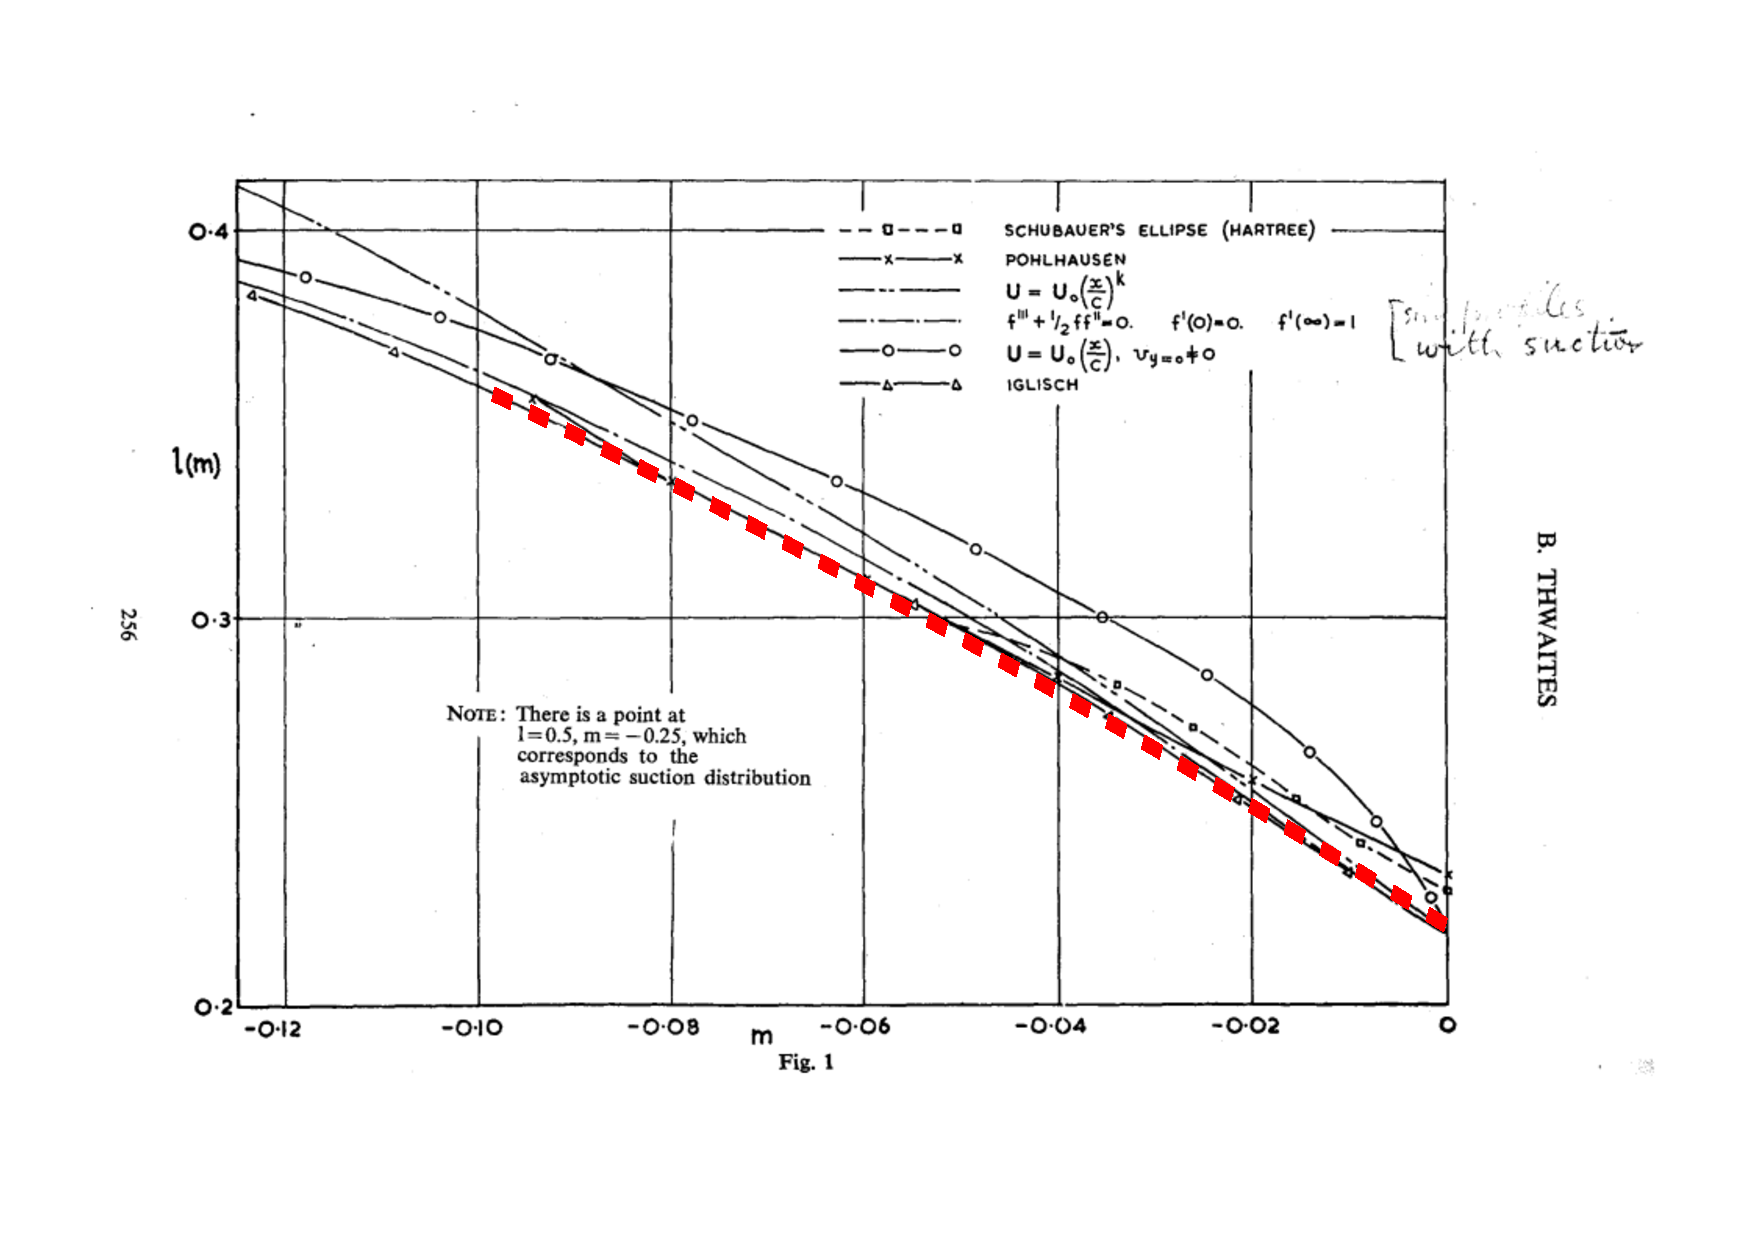
\includegraphics[width=0.95\textwidth, trim= 0  60 0  50, clip]{./../template/fig/cfr_ell_m_neg}
\caption{$\ell(m)$, per correnti accelerate, $m<0$.}\label{fig:ell_m_neg}
\end{figure}

\begin{figure}[h!]
\centering
 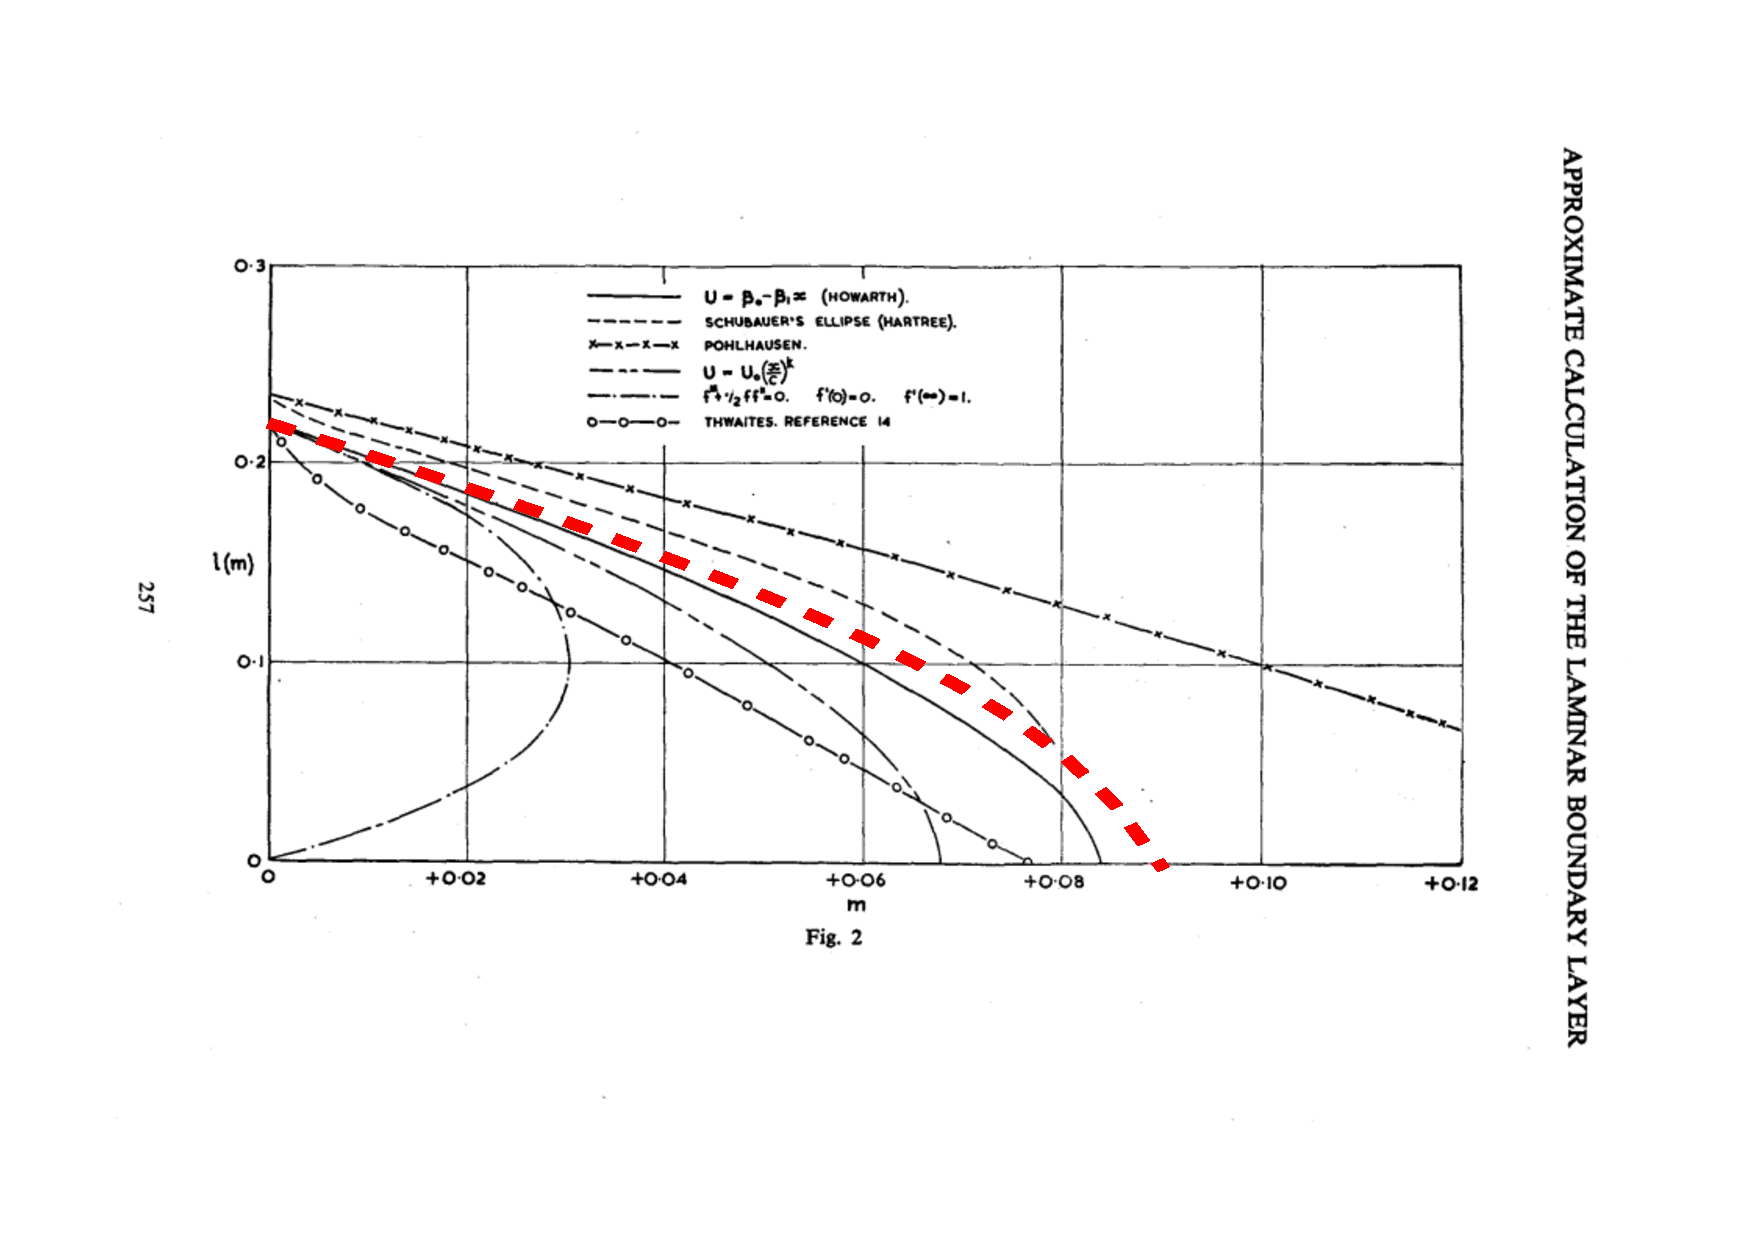
\includegraphics[width=0.95\textwidth, trim= 0  60 0 100, clip]{./../template/fig/cfr_ell_m_pos}
\caption{$\ell(m)$, per correnti con gradiente di pressione avverso, $m>0$.}\label{fig:ell_m_pos}
\end{figure}

\begin{figure}[h!]
\centering
 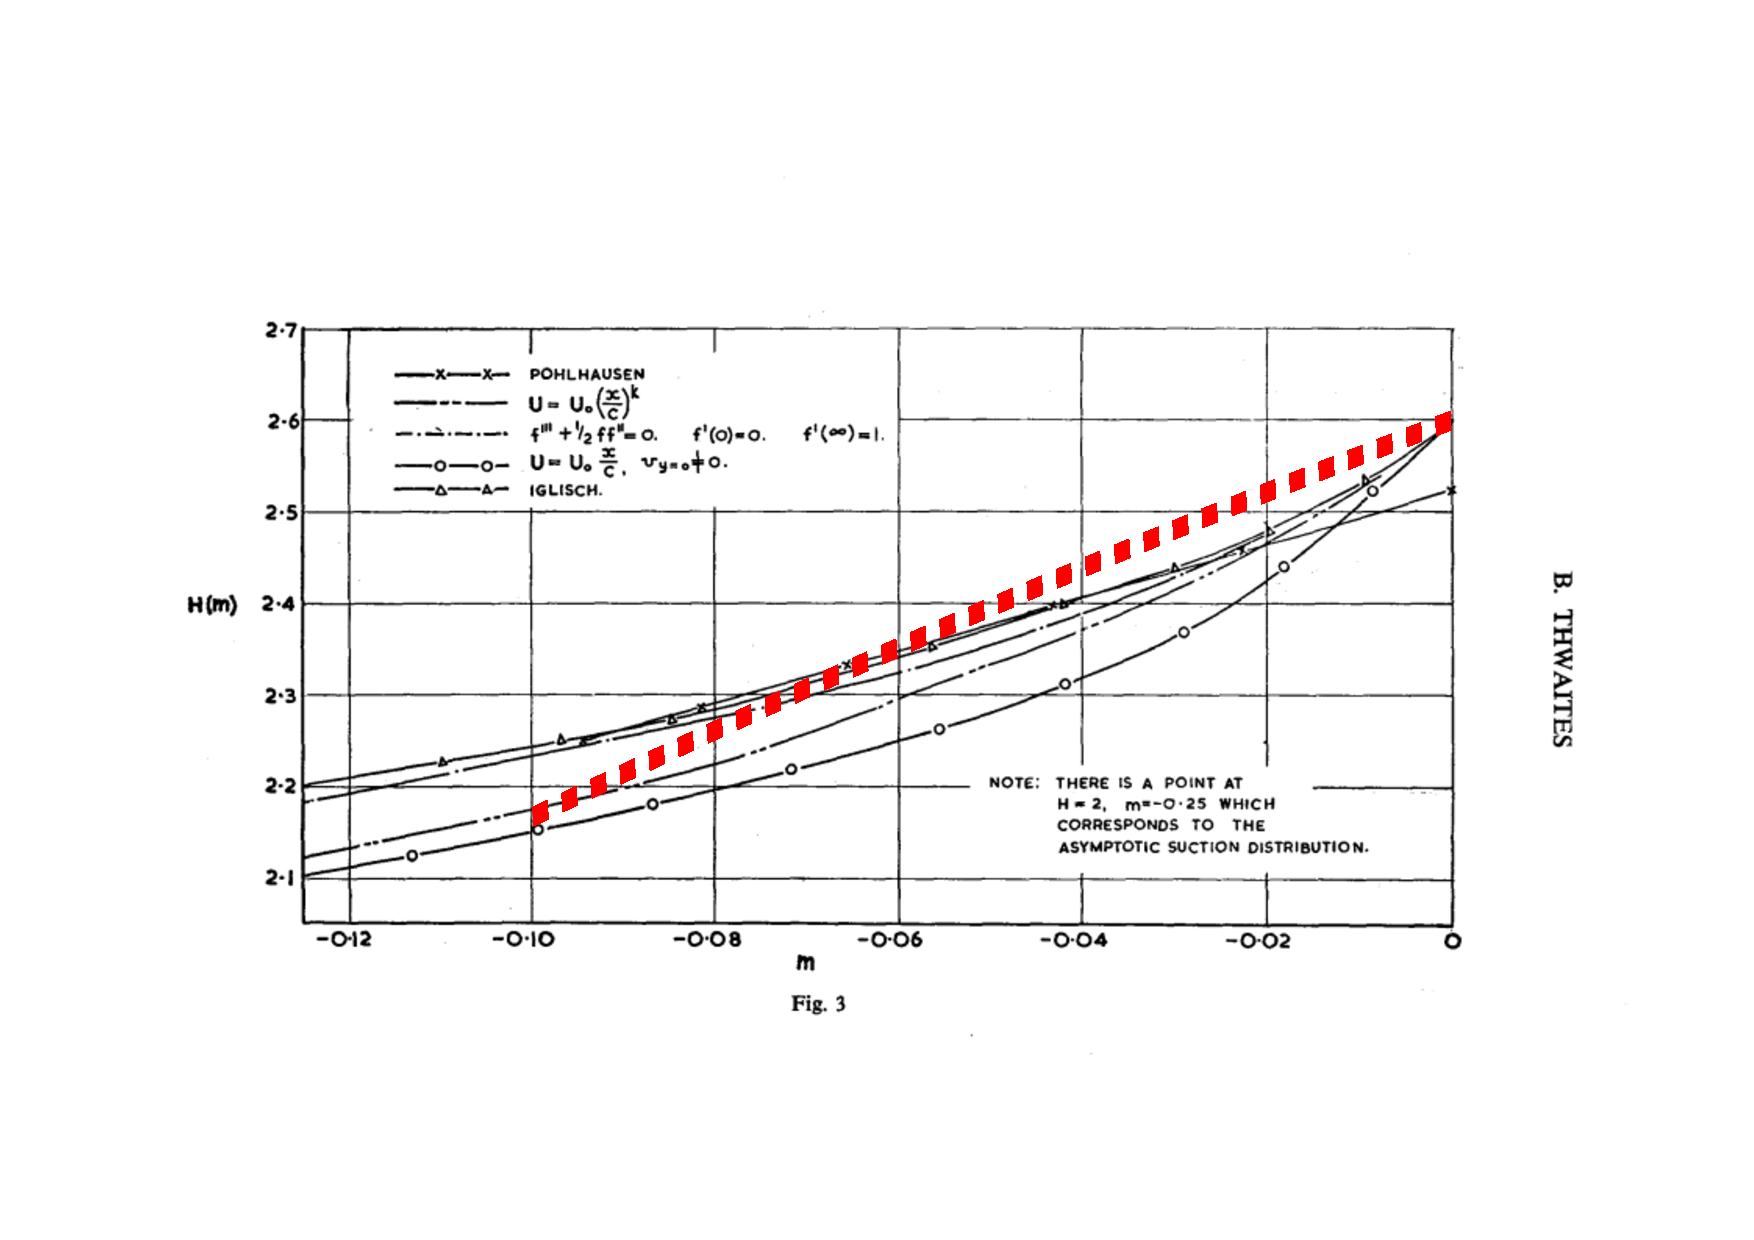
\includegraphics[width=0.95\textwidth, trim= 0 120 0 100, clip]{./../template/fig/cfr_H_m_neg}
\caption{$H(m)$, per correnti accelerate, $m<0$.}\label{fig:H_m_neg}
\end{figure}

\begin{figure}[h!]
\centering
 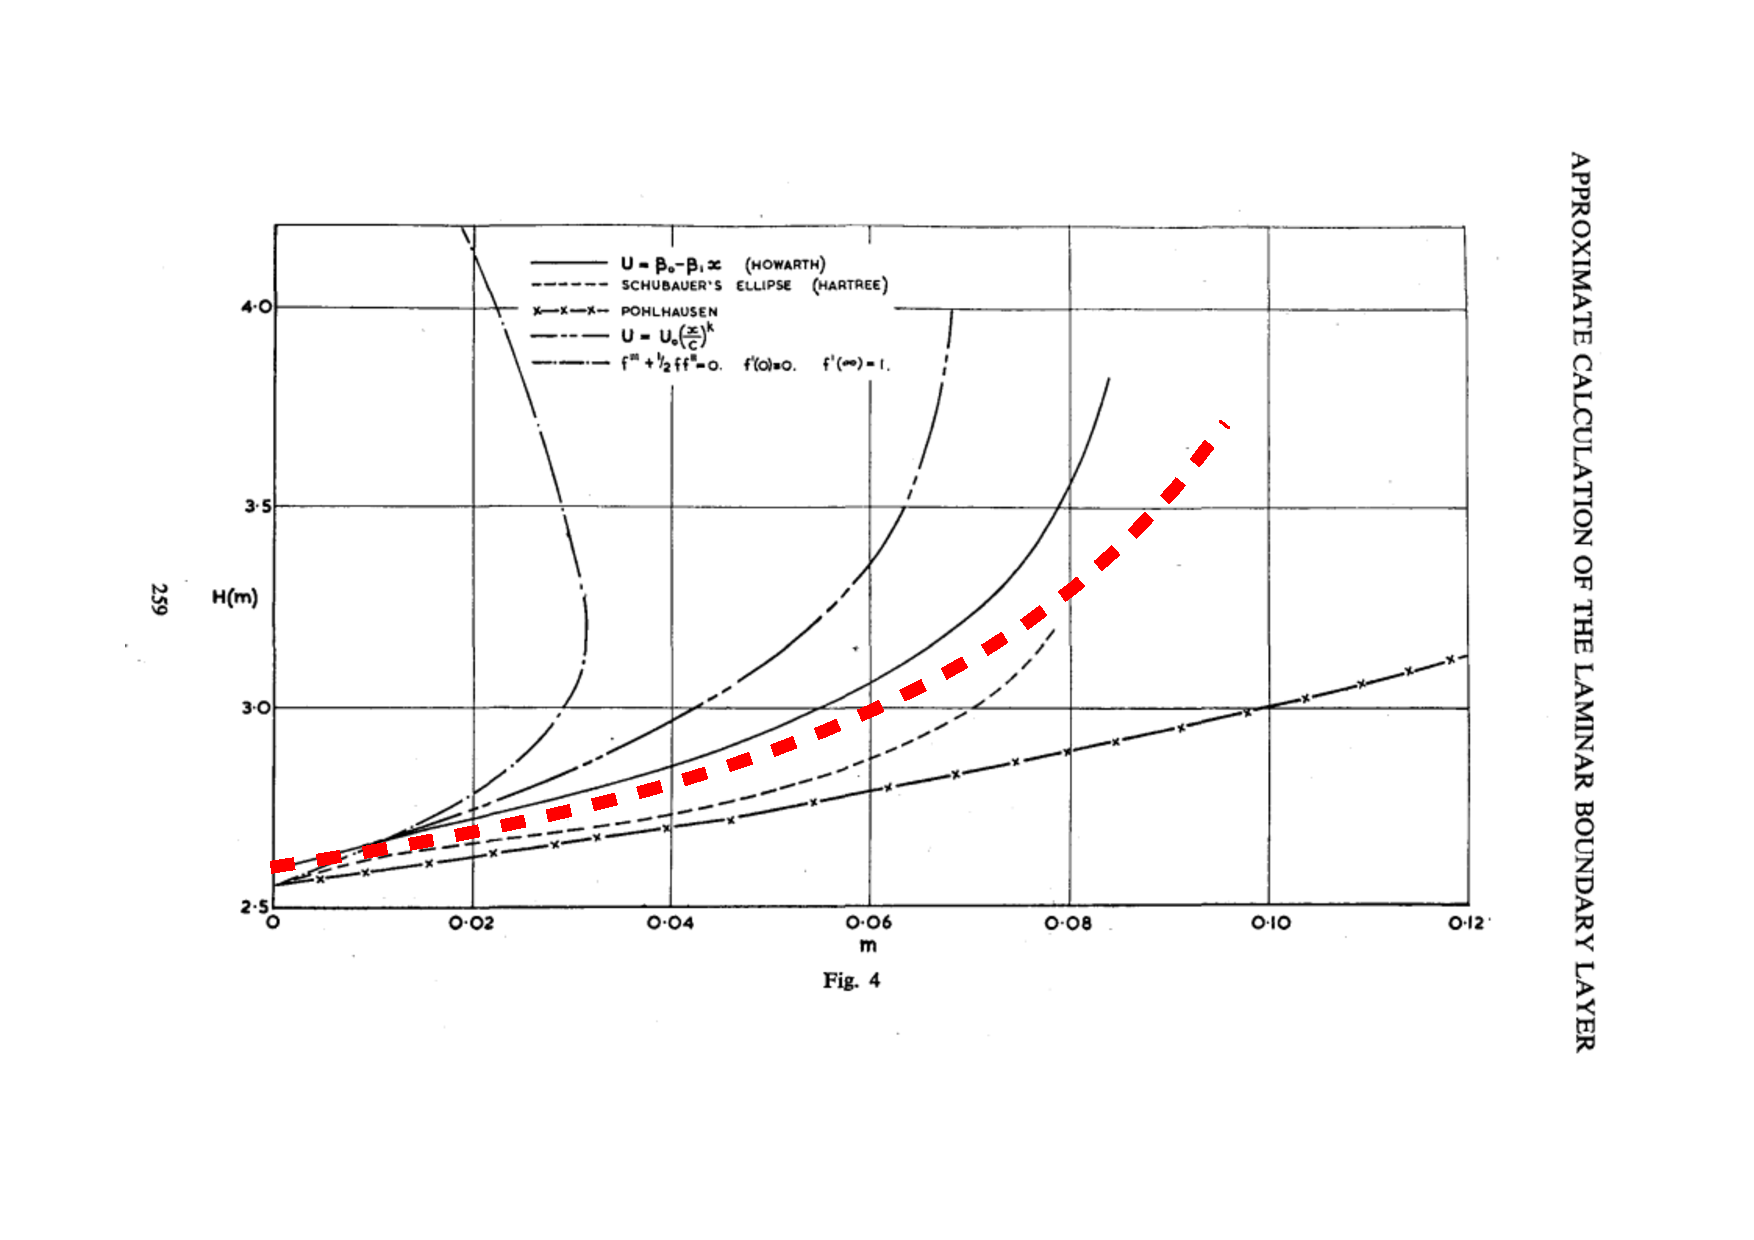
\includegraphics[width=0.95\textwidth, trim= 0  90 0 100, clip]{./../template/fig/cfr_H_m_pos}
\caption{$H(m)$, per correnti con gradiente di pressione avverso, $m>0$.}\label{fig:H_m_pos}
\end{figure}


\paragraph{Metodo di Thwaites ed equazione integrale di Von Karman.}
Si può manipolare l'equazione integrale di Von Karman (\ref{eqn:vkie}) per far comparire lo sforzo a parete $\tau_w$ e il gradiente di pressione $dP/dx$ prima, e i numeri adimensionali utilizzati da Thwaites $\ell$, $m$ poi.
%
Utilizzando la definizione del coefficiente di attrito,
\begin{equation}
 c_f := \dfrac{\tau_w}{\frac{1}{2}\rho U^2} \ ,
\end{equation}
e utilizzando il teorema di Bernoulli per legare la variazione della velocità esterna alla variazione della pressione,
\begin{equation}
 \rho U(x) \dfrac{dU}{dx}(x) = - \dfrac{dP}{dx}(x) \ ,
\end{equation}
si può riscrivere l'equazione di Von Karman come
\begin{equation}
\begin{aligned}
 \dfrac{d\theta}{dx} & = \dfrac{\tau_w}{\rho U^2} + ( 2 + H ) \dfrac{\theta}{\rho U^2}\dfrac{dP}{dx} = \\
  & = \dfrac{1}{\rho U^2} \left[ \dfrac{\mu U}{\theta} \, \ell + ( 2 + H ) \dfrac{\theta}{\rho U^2} \dfrac{\mu U}{\theta^2} \, m \right] = \\
  & = \dfrac{\nu}{U\theta} \left[  \ell + ( 2 + H ) \, m \right] \ .
\end{aligned}
\end{equation}
Secondo le ipotesi fatte da Thwaites, $\ell(m)$ e $H(m)$, il contenuto della parentesi quadra può essere scritto come una funzione di $m = \dfrac{dP}{dx} \dfrac{\theta^2(x)}{\mu U(x)}$,
\begin{equation}\label{eqn:vkie:2}
 \dfrac{U\theta}{\nu} \dfrac{d\theta}{dx} = [ \ell(m) + ( 2 + H(m) ) \, m ] =: \dfrac{L(m)}{2} \ .
\end{equation}
Conoscendo la distribuzione di velocità $U(x)$ e pressione $P(x)$ esterna, e l'espressione delle funzioni $\ell(m)$, $H(m)$, questa equazione contiene solo la funzione $\theta(x)$ come incognita, ed è integrabile (numericamente), una volta nota una condizione iniziale $\theta(x_0) = \theta_0$.

\paragraph{Linearizzazione di $L(m)$.} Nell'intorno di $m=0$, condizione di gradiente di pressione nullo, si può ottenere un'approssimazione affine della funzione $L(m)$,
\begin{equation}
 L(m) \approx 0.45 + 6 \, m \ .
\end{equation}
Inserendo questa approssimazione nell'equazione (\ref{eqn:vkie:2}), si ottiene
\begin{equation}\label{eqn:vkie:3}
 2 \dfrac{U(x) \theta(x)}{\nu} \dfrac{d \theta}{dx} = 0.45 - 6 \dfrac{\theta^2(x)}{\nu} \dfrac{dU}{dx} \ ,
\end{equation}
avendo espresso il parametero $m$ in funzione della variazione della velocità esterna,
\begin{equation}
 m = \dfrac{dP}{dx} \dfrac{\theta^2}{\mu U} = - \dfrac{\theta^2}{\nu} \dfrac{dU}{dx} \ .
\end{equation}
Moltiplicando l'equazione (\ref{eqn:vkie:3}) per $U^5(x)$, si può riscrivere
\begin{equation}
 \dfrac{d}{dx} \left( \theta^2 U^6 \right) = \nu U^5 \ ,
\end{equation}
pronta per essere integrata come
\begin{equation}
 U^6(x) \theta^2(x) - U^6(x_0) \theta^2(x_0) = 0.45 \, \nu \int_{\xi=0}^{x} U^5(\xi) d \xi \ ,
\end{equation}
da dove ricavare lo spessore integrale della quantità di moto $\theta(x)$.

\paragraph{Ricostruzione delle altre grandezze fisiche.}
Una volta calcolato $\theta(x)$, si può calcolare il parametro $m(x)$ lungo il corpo
\begin{equation}
  m = - \dfrac{\theta^2(x)}{\nu}\dfrac{dU}{dx}(x) \ ,
\end{equation}
con il quale calcolare gli altri parametri adimensionali,
\begin{equation}
 \ell(x) = \ell(m(x)) \qquad , \qquad H(x) = H(m(x)) \ ,
\end{equation}
con i quali calcolare lo sforzo a parete e lo spessore di spostamento
\begin{equation}
 \tau_w(x) = \ell(x) \dfrac{\mu U(x)}{\theta(x)} \qquad , \qquad \delta^*(x) = H(x) \theta(x) \ .
\end{equation}




% \vspace{10cm}
% 
% Utilizzando la definizione del coefficiente di attrito,
% \begin{equation}
%  c_f := \dfrac{\tau_w}{\frac{1}{2}\rho U^2} = 2 \dfrac{\nu}{U^2} \p{u}{y}\bigg|_{y=0} \ ,
% \end{equation}
% e la componente parallela alla parete della quantità di moto, valutata a parete,
% \begin{equation}
% 0 = \left[ u\p{u}{x} + v\p{u}{y} - \nu \dfrac{\partial^2 u}{\partial y^2} - U \f{dU}{dx}\right]\bigg|_{y=0} \qquad \rightarrow \qquad \nu \dfrac{\partial^2 u}{\partial y^2}\bigg|_{y=0} = - U \f{dU}{dx}  \ ,
% \end{equation}
% si può riscrivere l'equazione di Von Karman,
% \begin{equation}
%  \f{d\theta}{dx} - (2+H) \f{\theta}{U^2} \nu \dfrac{\partial^2 u}{\partial y^2}\bigg|_{y=0} =
%  \dfrac{\nu}{U^2} \p{u}{y}\bigg|_{y=0} \ ,
% \end{equation}
% e moltiplicando per il fattore $U \theta / \nu$,
% \begin{equation}
%  \f{U \theta}{\nu} \f{d\theta}{dx} =
%  \f{\theta}{U}\p{u}{y}\bigg|_{y=0} + (2+H) \f{\theta^2}{U} \dfrac{\partial^2 u}{\partial y^2}\bigg|_{y=0} \ .
% \end{equation}
% Seguendo Thwaites, vengono definiti due parametri adimensionali,
% \begin{equation}
%  \ell := \f{\theta}{U}\p{u}{y}\bigg|_{y=0} 
%  \qquad , \qquad
%     m := \f{\theta^2}{U} \dfrac{\partial^2 u}{\partial y^2}\bigg|_{y=0}
%        = - \dfrac{\theta^2}{\nu}\dfrac{dU}{dx} \ ,
% \end{equation}
% e l'equazione integrale di Von Karman diventa
% \begin{equation}
%  \f{U}{\nu} \f{d}{dx}\f{\theta^2}{2} = \ell + ( 2 + H ) m =: L(m) \ ,
% \end{equation}
% avendo introdotto la funzione $L(m)$, per la quale si può trovare una correlazione di dati sperimentali,
% \begin{equation}
%  L(m) = 0.45 + 6 \, m  \ .
% \end{equation}
% Utilizzando questa espressione della funzione $L(m)$ e la definizione di $m$ in termini della derivata della velocità esterna, l'equazione di Von Karman diventa
% \begin{equation}
%  \f{U}{\nu} \f{d}{dx}\f{\theta^2}{2} = 0.45 - 6 \f{\theta^2}{\nu}\f{dU}{dx} \ ,
% \end{equation}
% Portando a sinistra dell'uguale l'ultimo termine, moltiplicando tutti i termini dell'equazione per $U^5$, e sfruttando la regola di derivazione del prodotto, si può scrivere
% \begin{equation}
%  \f{d}{dx} \left( U^6 \theta^2 \right) = 0.45 \nu U^5 \ ,
% \end{equation}
% il cui integrale vale
% \begin{equation}
%  U^6(x)\theta^2(x) - U^6(x_0)\theta^2(x_0) = 0.45 \nu \int_{\xi=0}^{x} U^5(\xi) d\xi \ .
% \end{equation}
% Se si integra questa equazione a partire da un punto $x_0$ dove la velocità esterna è nulla, $U(x_0)^2$, si può trovare l'andamento dello spessore integrale della quantità di moto,
% \begin{equation}
%  \theta^2(x) = 0.45 \nu \f{1}{U^5(x)} \int_{\xi=0}^{x} U^5(\xi) d\xi \ .
% \end{equation}
% 

\clearpage \newpage


\end{document}
